\documentclass[whitelogo]{tudelft-report}
\usepackage{natbib}
\usepackage{changes}
\usepackage{amsthm}
\usepackage{algorithm}
\usepackage[noend]{algpseudocode}


\theoremstyle{plain}
\newtheorem{thm}{Theorem} % reset theorem numbering for each chapter

\theoremstyle{definition}
\newtheorem{defn}[thm]{Definition} % definition numbers are dependent on theorem numbers
\newtheorem{exmp}[thm]{Example} % same for example numbers

\begin{document}

%% Use Roman numerals for the page numbers of the title pages and table of
%% contents.
\frontmatter

%% Uncomment following 19 lines for a cover with a picture on the lower half only
%\title[tudelft-white]{Title}
%\subtitle[tudelft-cyan]{Optional subtitle}
%\author[tudelft-white]{J.\ Random Author}
%\affiliation{Technische Universiteit Delft}
%\coverimage{cover.jpg}
%\titleoffsetx{10cm}
%\titleoffsety{10cm}
%\afiloffsetx{1cm}
%\afiloffsety{18cm}
%\covertext[tudelft-white]{
%    \textbf{Cover Text} \\
%    possibly \\
%    spanning 
%    multiple 
%    lines
%    \vfill
%    ISBN 000-00-0000-000-0
%}
%\makecover

%% Uncomment following 16 lines for a cover with a picture on the lower half only
% \title[tudelft-white]{Towards global consensus on trust}
% \subtitle[tudelft-black]{Aggregation of temporal PageRank trust vectors}
% \author[tudelft-white]{J.\ Harms}
% \affiliation{Technische Universiteit Delft}
% \coverimage{cover.jpg}
% \setpagecolor{tudelft-cyan}
% \makecover[split]


%% Include an optional title page.
% \begin{titlepage}


\begin{center}

%% Insert the TU Delft logo at the bottom of the page.

%% Print the title in cyan.
{\makeatletter
\largetitlestyle\fontsize{64}{94}\selectfont\@title
%\largetitlestyle\color{tudelft-cyan}\Huge\@title
\makeatother}

%% Print the optional subtitle in black.
{\makeatletter
\ifx\@subtitle\undefined\else
    \bigskip
   {\tudsffamily\fontsize{22}{32}\selectfont\@subtitle}    
    %\titlefont\titleshape\LARGE\@subtitle
\fi
\makeatother}

\bigskip
\bigskip

by
%door

\bigskip
\bigskip

%% Print the name of the author.
{\makeatletter
%\largetitlefont\Large\bfseries\@author
\largetitlestyle\fontsize{26}{26}\selectfont\@author
\makeatother}

\bigskip
\bigskip

to obtain the degree of Master of Science
%ter verkrijging van de graad van Master of Science

at the Delft University of Technology,
%aan de Technische Universiteit Delft,

to be defended publicly on Tuesday January 1, 2013 at 10:00 AM.
%in het openbaar de verdedigen op dinsdag 1 januari om 10:00 uur.

\vfill

\begin{tabular}{lll}
    Student number: & 1234567 \\
    Project duration: & \multicolumn{2}{l}{March 1, 2012 -- January 1, 2013} \\
    Thesis committee: & Prof.\ dr.\ ir.\ J.\ Doe, & TU Delft, supervisor \\
        & Dr.\ E.\ L.\ Brown, & TU Delft \\
        & Ir.\ A.\ Aaronson, & Acme Corporation
\end{tabular}
%% Only include the following lines if confidentiality is applicable.

\bigskip
\bigskip
\emph{This thesis is confidential and cannot be made public until December 31, 2013.}
%\emph{Op dit verslag is geheimhouding van toepassing tot en met 31 december 2013.}

\bigskip
\bigskip
An electronic version of this thesis is available at \url{http://repository.tudelft.nl/}.
%\\[1cm]

%\centering{
\includegraphics{cover/logo_black}}


\end{center}

\begin{tikzpicture}[remember picture, overlay]
    \node at (current page.south)[anchor=south,inner sep=0pt]{
        
\includegraphics{cover/logo_black}
    };
\end{tikzpicture}

\end{titlepage}



% \chapter*{Preface}
\setheader{Preface}

The big hype around Bitcoin and other cryptocurrencies seems to create a distorted picture of the 
original idea of a distributed, democratic financial system. The general public does not appreciate
the simplicity and brilliance of the concept but rather the price swings and the
possibility to become rich. 

A similar distortion happened to the internet itself. Once envisioned as an 
open and free network for information exchange, the World Wide Web has been transformed into an
infrastructure for commerce, data collection and cyber attacks. Certainly, many companies have created 
solutions that simplify our lives significantly. But the free use of all kinds of services comes at 
an invisible cost. Slowly, that cost becomes more visible as targeted misinformation campaigns are
dismantling democracies and data collection policies of the big internet monopolies are uncovered.

Decentralization is a natural solution to this problem. Some fundamental services such as transferring
money, communication and the access to information should not be controlled by single entities and 
exploited for profit. In the same sense, creating trust with other internet users should be 
enabled through a decentralized system. This is the motivation to contribute to the design of a
distributed trust system.

Working on this thesis has been a journey through many fields of science, from evolution theory and 
social sciences to synchronization methods of replicated databases. 
It has in many ways opened my eyes to the problems of centralized 
organizations and the advantages that distributed systems offer. Also, it sparked my interest in 
trust, cooperation and their relation to problems of society.

I would like to thank my supervisor Dr.\ Johan Pouwelse for his enthusiasm, infinitely large pool of
ideas and suggestions as well as his invaluable feedback. I thank the Tribler team for keeping me 
awake with coffee and the review work of Quinten and Martijn. I thank my parents, my girlfriend, Lyla, 
and my closest friends for their support in moments of self-doubt. A special thanks goes to my 
housemates Marnix and Liesette who helped me through the last weeks. I would also like to thank 
Alexander for our interesting talks at lunch. Without you it wouldn't have been possible.


\begin{flushright}
{\makeatletter\itshape
    \@author \\
    Delft, August 2018
\makeatother}
\end{flushright}



% \tableofcontents

%% Use Arabic numerals for the page numbers of the chapters.
\mainmatter

\chapter{Introduction}
\label{chap:introduction}
% \subtitle{Building a distributed reputation system as the basic infrastructure for creating trust 
% between relative strangers for the future digital economy.}

% \paragraph{Abstract.} Trust enables cooperation which in the long-term increases welfare for all 
% parties, but centralization creates an unhealthy information and, thus, power asymmetry. The future 
% digital economy will be driven by global cooperation between relative strangers; that cooperation 
% will be facilitated by distributed reputation systems without central ownership or control. This 
% work extends the scalable TrustChain fabric with an explicit, unambiguous, public representation of 
% the entities' states, thereby making sharing of information incentive-compatbile and putting another
% pillar for the trustful internet in place.

% 1. Since the ground-breaking work of Darwin we know that evolution of species is guided by natural selection, so mutation and inheritance lead to the strongest variation surviving. However, the classic view of the strongest survives does not explain how cooperation can occur, which requires some sort of altruism. Game theory explains …
%  Nowak, Axelrod, 

Trust is the bedrock of society. From the evolution of species, global markets all the way to the 
modern sharing economy, trust has always had an important impact on almost every aspect of our lives.
Trust is built on a good reputation which in turn is created through positive outcomes of past 
interactions. The value of a good reputation also depends on how widely known that reputation is.
In small communities, knowledge about each other is gained through gossiping or personal experience. 
But local communities become less important as global communities and marketplaces become more common
through internet based applications. Still, or even more so, those internet communities depend on 
trust. Protecting and distributing the knowledge about interactions in the digital world is a tough
challenge we are faced with when designing a global trust system.

The current state-of-the-art trust building systems are online platforms for the sharing economy.
The reputation systems of Uber\footnote{https://uber.com} and AirBnB\footnote{https://airbnb.com} are
an essential part of their business. The good reputation allows commuters to trust their driver and
get into the car of a stranger, or allows house owners to rent their home to a couple from the other
side of the world. The reputation of drivers and renters are stored on the platforms, they are both
valuable to the people as well as the company. This leads to problems when renters do not agree with
updates to the platform: they cannot take their reputation and move to a competitor. Users are locked
into those platform, giving platforms great power and influence. 

A similar situation exists in the banking world. Banks are entrusted with their clients money, but 
their power led to corruption and the trust was abused. The situation escalated in the 2007-08 
financial crisis which led to a global recession. The crisis inspired a new solution: Bitcoin. Bitcoin
is supposed to enable secure payments without banks. As such it removes power from financial 
institutions and puts it back into the hands of the actual owners of the money. 

Not every digital money transaction should require a bank, and similarly not every trustful
interaction on the internet should require a third-party. Instead, the ability to prove one's trustworthiness
on the internet should be open and free for anyone. Our vision is therefore to create a universal
mechanism to create trust. This work sets an important 
step towards creating such a system. Specifically we propose a mechanism that protects and 
distributes the records of transaction which are essential for creating trust. 

This first chapter introduces some key concepts around trust and explains the context of this work.
It should shed light on the origin of trust research and its significance for the future of the 
internet. A thorough contextual basis is created for the reader to fathom the problem description
and proposed solution in the following chapters.

\section{Trust research}
Virtually everyone that is part of a social community understands the concept of trust, yet defining
trust scientifically is hard. This is also due to the fact that trust is studied in a diverse set 
of sciences: evolutionary biology, sociology, economics and lately computer science. In the simplified
form of a model trust can well be described and studied. The prisoner's 
dilemma\cite{chammah1965prisoner} is one such model from game theory that creates a framework for 
understanding trust. It is widely used in research and is the basis for many experimental studies.
We describe in the following the game, it's relation with cooperation and the impact on evolutionary
theory, economics and computer networks.

\subsection{Prisoner's dilemma}
\label{sec:prisoner}
The game Prisoner's dilemma describes a dilemma common in many real-world situations, for
example the problem of two partners caught for a crime that are questioned in two separate rooms. 
Each prisoner has two options, either deny all allegations, which is more generally called cooperating
 or betray the partner, which is called defecting in general game theory. If both stay 
silent, both will get a sentence of one year. If one betrays the other, the snitch is set free while the 
betrayed gets three years in prison. If both betray each other, they both have to serve two years.
When analyzing the game without any additional knowledge and considering the payoffs for one of the
prisoner's it is always advantageous to betray the other. Either the other also betrays, in which case
two years is better than three, or the other stays silent in which case betraying sets us free. 
However, when considering both prisoners' outcomes together it would be best for both to stay silent.


While the game is quite simple the implications are far reaching. The game is able to show the 
connection between trust and cooperation. If both prisoners trust each other to never betray a 
partner, both will cooperate and get a small sentence, the best combined outcome. Yet any mistrust
makes both fail at beating the system. The problem also describes many real world problems, called 
the tragedy of the commons. For example, the global warming is a problem that can only be solved if
all peoples and all nations cooperate. Yet, the low cost and convenient usability of fossil fuels 
make it advantageous to defect and damage the environment. Either the others try to save the environment
in which case a single defection will have a small impact, or the other will also damage the environment
in which case a single cooperator will fail anyways. Only, if everyone trusts each other that
everyone does the best they can to save the environment, then it is possible to beat the tragedy 
of the commons.

\subsection{Evolution and cooperation}
\label{sec:evolution}
While cooperating, according to theory, is not necessarily a winning strategy, it is in our nature 
to do so, as has been shown by evolution theorists. The theory about competitive natural selection 
between individuals and mutation and inheritance of genes was the accepted truth about evolution 
since Darwin until in the late 1960s doubts arose about the completeness of this 
theory. When looking at group behavior in species one will find that cooperation is a common theme
among related individuals, yet there is no place for cooperation in the classic Darwin 
theory~\cite{Axelrod1390}. In their work Axelrod and Hamilton \cite{Axelrod1390} 
analyze how to combine the seemingly inferior individual's strategy of cooperating with the goal to 
maximize fitness. At the basis of their experiments is a again the Prisoner's 
Dilemma. Axelrod and Hamilton ran experiments on this game with multiple rounds instead of only one with
different strategies. They found that if the game is played repeatedly with the possibility of 
meeting the same partner again in the future, cooperation between players can be established and be
superior. Later research showed that this direct form of reciprocity, the act of returning a deed,
is only one form of cooperation found in human behavior. Nowak and 
Martin~\cite{nowak2006five} defined in total five forms in which cooperation can occur: kin selection, direct
reciprocity, indirect reciprocity, network reciprocity and group reciprocity. Conceptually these 
forms can be described like this:

\begin{itemize}
    \item kin selection: we help those that share our genes
    \item direct reciprocity: I help you, you help me
    \item indirect reciprocity: I help you, somebody helps me
    \item network reciprocity: neighbors help each other
    \item group selection: A group, in which members help each other, survives
\end{itemize}

Each concept entails at its basis trust. We trust our family, our group, our countrymen, those with whom we had a lot
of shared experiences and those we heard good things about. 
% 2. Trust in economy and digital markets …. Advance of sharing economy, ….. When talking about trust, indirect reciprocity is the method of creating cooperation. Mui created a first mathematical model which relates reputation, trust and reciprocity. According to that model reputation stems from the history of encounters 
% Mui, Martin

\subsection{Economics}
{\color{red} Old: needs to be improved}
Trust also plays a major role in our economic system and has been for the the evolution of economy 
as shown in Figure \ref{fig:economy}. In the pre-industrial age, most economy and trade was done in local
communities with families that trusted each other over generations and traders that returned year
after year. During industrial and post-industrial age companies have largely replaced local 
producers and are trusted by millions of customers based on their brand name. Nowadays, in the 
information age, internet companies allow people to connect, trade and cooperate directly, examples
being eBay for trading physical goods, AirBnb for sharing houses and Uber for ride-hailing. How trust
and the lack of it influence trade and markets has been studied in the well-known paper by 
Akerlof~\cite{akerlof1970lemons}. He describes the information asymmetry between seller, who knows
the quality of the goods which will be sold, and the buyer, who can only estimate that quality by 
some market statistic. The seller's incentive to sell goods of lesser quality than the average 
statistic leads to a decreasing statistic and thus price which in turn decreases the quality of the 
goods sellers are willing to offer for that lower price. Hence the market breaks down. Akerlof
describes institutions to solve this problem namely institutions such as guarantees, brand names and
certifications. These are trust inducing institutions and can be generalized as reputation systems.
If the sellers sell goods to many people and those people report or gossip the good quality of what
they have bought, others can trust those sellers and both seller and buyers will thrive. On the 
other hand a bad reputation will lead to a seller getting out of business as buyers will mistrust.
This closes the gap to the work of Nowak as this reputation is what makes indirect reciprocity
possible: the seller is not taking advantage of the buyer's inconvenient situation but the buyer
cannot directly return that favor. Only by gossipping the event to other potential buyers who are 
then more willingly to buy from the seller is the reciprocity circle closed.~\cite{nowak2006five}

\begin{figure}[t]
    \centering
    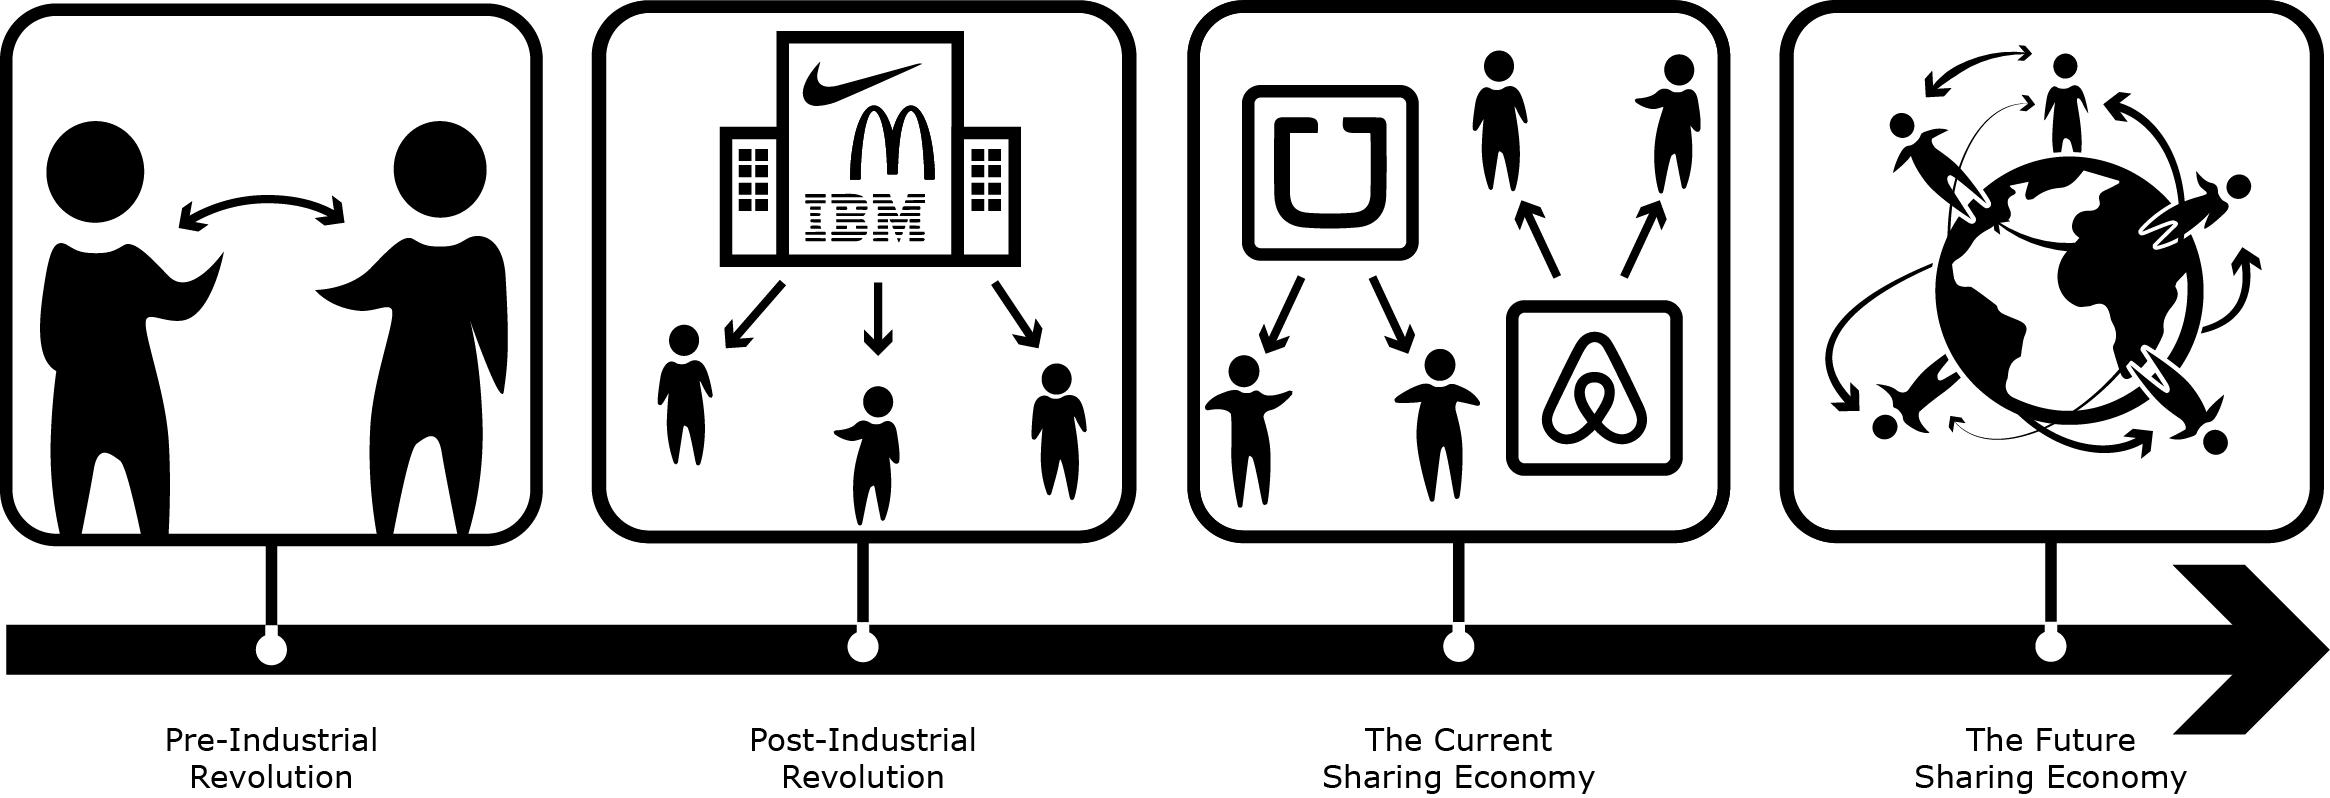
\includegraphics[width=0.8\textwidth]{images/economy.png}
    \caption{Evolution of the economy}
    \label{fig:economy}
\end{figure}

% 3. Reputation systems guide buyers towards to most trustworthy sellers on markets or help guests find houses on Airbnb that actually hold the promises made in the description. Reputation systems require three properties: dissemination, strong identities and  Yet companies take advantage of our trust and misuse our data, influence us and do not take appropriate measures to protect our data from attacks. Centralized systems are broken.
% (eBay) Ba and Pavlou, survey of reputation systems, definition of reputation system, Pouwelse 
\section{Digital trust}
{\color{red} Old: needs to be improved}
These analog, gossip-based reputation systems are what guide our decisions in buying cars, new or 
used, at which bank we store our money and at which restaurant we should have dinner.
But reputation systems are also prevalent in the digital world: we make our decisions in buying used goods 
on eBay, renting a house to a stranger (or from a stranger), getting into a stranger's car 
(what mum told us not to) based on the reputation of the partner. The sharing economy or collaborative consumption is the 
rising star of economic concepts in the information age and it is power by reputation. A company 
offers a platform on which the two sides of a trade or transaction can find each other. With each 
encounter both parties can rate that interaction and it becomes part of their history. With a longer
and more positive history the value of a profile increases as users see the reputation as security
for a good interaction and are willing to pay for it. However, there are reasons for concern. What
if the platform changes their rules in an almost unacceptable way or abuses the personal data their
users have entrusted them with? Users cannot take their reputation and data to another platform
because their reputation is actually owned by the platform facilitating the trades. Such abuses
in which trusted companies act wrongly have been happening in many times in the past, examples being
the dieselgate~\cite{VWDiesel} and the facebook/cambridge analytica scandals.~\cite{facebook} These
scandals show that even though millions of users trust them, central institutions do not necessarily
serve their customers or clients. 

% 4. The above discussion makes clear that the future digital economy requires a distributed reputation system. But making a reputation system distributed brings many additional challenges. A distributed system has no control entity which can enforce strong evidence for identities. Also single entities in a distributed system have most commonly no full view of the network, thus are not aware of all other entities or all encounters. The field is not entriely new but distributed reputation systems have been researched especially in the context of peer-to-peer file-sharing, and mobile ad-hoc system. Donation game is the game-theoretic model for this …. Although a lot of research has been conducted in the field of distributed reputation systems, major problems like the Sybil-attack, double spending, scalability and state consistency remain largely unsolved.
% Game-theoretic modeling of reputation
\section{Universal mechanism to create trust}
{\color{red} Old: needs to be improved}
We envision a future in which collaborative consumption is possible without any intermediator. This
future requires a reputation system which is application agnostic, owned by noone and ruled by 
everyone. A distributed reputation system as a layer directly
on top of the internet. However this poses some challenges from a technical
point of view. Distributed system are intrinsically hard to control and regulate, which is both 
blessing and curse. No party can impose unfair rules on other users but it is also hard to prevent 
malicious users from sending wrong information across the network. \cite{HENDRIKX2015184} reviews
state-of-the-art reputation systems and finds that all commercial reputation systems are centralized.
Some of the scientific reputation systems are decentralized like EigenTrust 
\cite{kamvar2003eigentrust}, P-Grid \cite{aberer2003p} and RateWeb \cite{malik2009rateweb}, yet
they have not been proven to work in settings where high throughput, global scaling are required 
which is the case for a global reputation system. Distributed, secure and globally scalable systems
remain an unsolved problem.

% 5. This master thesis was written in the context of the blockchain lab at TU Delft which has a long history of research on the topic of distributed reputation systems. The research is targeted at Tribler, a secure BitTorrent client which is aimed at protecting against free-riders.
% BarterCast

\section{TU Delft Blockchain Lab research}
The ambition of creating the first global trust system is realized at the Blockchain Lab of TU Delft,
which is the research group in which this thesis was created. The lab has a strong focus on exploring
new concepts, implementing them and testing them in production grade software. 

The research group has great experience and a solid track record in the field of distributed work 
systems. Especially peer-to-peer file sharing system have been studied, first and foremost the 
internally developed Tribler\footnote{https://tribler.org} application. Tribler is a client for the
BitTorrent protocol. It offers many improvements over conventional BitTorrent clients like improved
privacy and security, streaming and reputation management. It has been the testbed for algorithms of
bachelor, master and Phd students for ten years with 1 million downloads in that period. In those 
years of research several milestones have been reached. In \cite{meulpolder2009bartercast} we have 
solved the free-riding problem in the peer-to-peer file-sharing context with a reputation system 
that tracks uploads and downloads. With TrustChain \cite{OTTE2017} we have created our own 
blockchain fabric for bandwidth as a currency which builds on the previous work and adds 
tamper-proof recording and immutable history to the reputation system.

The problem of peer-to-peer file sharing systems maps well onto the trust domain. Users of BitTorrent
clients download from other users who upload data. Downloading data has benefit to users because 
they are interested in the content, however uploading has no obvious advantage. It is only necessary
to keep the content available for others. There is an obvious incentive problem, a tragedy of the 
commons. A free-rider can download without uploading, thereby consume resources without contributing.
The problem can be solved through a trust system. By recording the behavior of each user and making
it public a reputation can be assigned to each user which represents their resource usage. Users 
that contribute a lot increase their reputation while downloading decreases that reputation. Other 
users are able to inspect that past behavior of any potential partner and use it for their decision 
whether the partner deserves a contribution. 

The recording of file transactions and security of those records is facilitated by our blockchain
fabric TrustChain~\cite{OTTE2017}. TrustChain is a multi-chain fabric which lets each user create
an own chain. It is therefore built for horizontal scalability and unbounded throughput. By design,
TrustChain enables the creation of trust in any application context. The solution is implemented
in Tribler and has been used in production for more than a year as of 2018. The implementation 
details of TrustChain will be discussed more in Chapter~\ref{chap:model}. 

The great scalability of TrustChain comes at the cost of security. The architecture allows for 
attacks to be detected but the system can only be secured if honest users engage in that defensive 
behavior. This can only be ensured through incentives: agents should never be able to gain an 
advantage by circumventing the rules. 

\section{Contribution}
In this work we study a mechanism to ensure the proper dissemination and verification of transaction
records. In any trust system, the transaction records are the basis for the reputation of users and 
thus the trust users have in each other. With the records, also the reputations itself are spread, 
leading to more agreement of reputation and thus higher value. Also defending the reputation records
against attacks makes records more credible and dependable, opening applications for TrustChain with
higher requirements for security.

We will enlarge on the problem description in the next chapter. Afterwards the problem will be defined
formally and analyzed in the bounds of the definition. Before proposing a solution, some existing
approaches for recording and dissemination of data will be discussed in chapter. Next, we define a
solution based on the TU Delft blockchain fabric TrustChain and propose a specific mechanism of 
using such a fabric. Finally, we prove the correctness and scalability properties of the fabric in
experimental analysis, before concluding and making suggestions for further research.

\chapter{Problem description}
In the introduction we make a case for the decentralization of applications that handle private
information or resources and argues that scalability is one of the main problems of the promising
blockchain technology to make such systems a reality. Trustchain is an approach that removes the 
main bottleneck that restricts the scalability of the most common blockchain fabrics, namely global
consensus. However the lack of agreement on a single accepted set of transactions has many 
implications for attack resistance and correctness guarantess of the system. This chapter 
introduces these implications and defines the problem that this work is supposed to tackle.

\section{Attacks}

\subsection{Double-spend attack}
One of the most challenging attacks that exist in distributed systems is the \textit{double-spend}
attack in which an adversary creates two conflicting transactions with two different agents without
telling each about the other, effectively using resources twice. In centralized systems this attack
is prevented by the central server which processed transactions in order and realizes that the 
resources were spent in the first version of the transaction. Bitcoin was the first decentralized
accounting system that solved this problem without a central, trusted entity. However the mining
which creates a single accepted sequence for transactions is costly in terms of time and resources.
Without global consensus Trustchain (discussed in more detail in section 3) is not able to prevent 
the double-spend attack. Instead, the double-spend attack will be recorded and therefore made 
detectable. The attacker sends two conflicting transactions to two different agents and keeps one,
but both partners write the conflicting blocks on their chains. If those two agents share their 
blocks with each other or both share their blocks with a third agent, the attack becomes detectable
because the two blocks are conflicting. The prevention of this attack therefore requires 
dissemination of transaction data across the network and constant checking for conflicting 
transactions by all agents.

\subsection{Sybil attack}
During a sybil attack an adversary takes control over many entities at the same time without making
this known to the network. The attacker can then use those entities to gain influence without any
real cost because the controlled entities can create proof of transactions without actually 
performing them.

This problem is very hard to detect because controlled entities can look like real agents to 
external observers. In centralized systems this is often prevented by requiring multiple 
authentication steps, for example scanning an identity card. Also if the creation of new agents has
some costs, the adversary needs to evaluate the possible advantage against the cost of creating
multiple agents.
In Bitcoin and other proof-of-work based cryptocurrencies the attack is avoided because the power
to create a new block is proportional to computational power, so whether the computational power
is spread over multiple agents or not does not matter to the voting power in the system.

For other decentralized systems the sybil attack continues to be a challenging problem. Many 
solutions have been proposed which analyze the topology of the network. Also an initial negative 
balance has been proposed by some. Specifically for the Trustchain two algorithms, namely NetFlow
and Temporal PageRank. Yet, while the two algorithms allow for sybil-resistant calculation of a 
metric which is related to the balance of agents. Also the accuracy of the algorithms depends on 
the amount of data that is available, making it neccessary to share data between agents in order
to better be able to estimate the probability of sybils. The sybil attack will further be discussed
in chapter 4.

\subsection{Blockwithholding attack}
In decentralized systems it can be advantageous for agents to not share some information about
their transactions that would otherwise render them in a weaker position. This is not possible
in centralized systems because users do not keep their own data which instead is stored on the
central server. Thus it is not the user's decision to share or not share information with others.

In common blockchain fabrics all information is shared with everyone and only information that is 
accepted by everyone is true. By removing the global consensus this guarantee is no longer intact.
If user's own their data, they can decide to share it or not. Agents can claim that information was
lost during transactions or that a transaction did not take place.

\subsection{Dishonest behaviour}
Some application types may require agents to act according to a specific set of rules. For example
in the Tribler application, if an agent (responder) receives two requests for contribution the 
agent should contribute to the one agent that has contributed the most in the past as that agent 
deserves to be rewarded for those past contributions. Without global consensus the agent determines
the ``goodness'' of the requesters on the basis of an unobserved information set, which is a subset
of the global network information. However the agent can also decide to not stick to the rules and
contribute to the lesser of the two requesters. Without consensus on the information set on the 
basis of which the responder decides, this dishonest behaviour cannot be detected and punished by
other agents.

\section{Research question}
From the above discussion it becomes clear that removing the global consensus from any blockchain
farbics opens the system to many forms of attacks. The missing guarantees on information makes it
hard to check the correct behaviour of other agents. This makes sharing of information and 
validation of transactions an essential building block of a blockchain system without global
consensus. Yet, the question is how to enforce dissemination of transaction records without a
trusted third party. Also which information is neccessary to distribute accross the network and how
can we make sure that validation of that information is done by all nodes. Formally we can define 
the following research question:

\begin{center}
    \textit{How can we design a scalable, decentralized accounting system that ensures the distribution,
    correctness and honest usage of transaction records?}
\end{center}

The research question entails some requirements for the system that we are trying to develop. In 
the following we will explain each of those in more detail.


\subsection{Accounting system}
\label{sec:accounting_system}
The system we are trying to build is an accounting system. An accounting system keeps track of 
transactions of a resource of value between at least two parties. Accounting systems have many 
applications; two common examples are a banking system and a reputation system. Each entity in 
the accounting system has a unique identifier and from the history of the transactions recorded 
in the system a certain balance can be assigned to each identifier. When a new transaction is issued 
the balance is increased or decreased and usually some threshold is put inplace to restrict the 
infinite spending of resources. This implies that the order of transactions is of importance. As an 
example consider an entity A with the balance of 5 a minimum threshold of 0 and two transaction 
spending 4 units and 3 units two parties B and C, respectively. Obviously, it is not possible that
both transactions are accepted. Either, A first spends 4 units on the interaction with B and cannot
afford the transaction with C or the other way around. If entity A tries to submit both transactions
at the exact same time, it is the task of the accounting system to create an order of two transactions
and restrict the expenditure beyond the balance threshold.

\subsection{Scalability}
Accounting systems can exist in many different sizes and contexts, they do not even have to be
digital for some applications. However in this work we are concerned with planet-scale accounting
which even enables micro-transactions with high frequency. Therefore scalability is one of the 
main factors. Before the ascent of internet applications such dimensions were unheard of but in
the last decade services such as Facebook, WeChat or YouTube have shown that an application can 
grow to have billions of users. Our ambition is to lay the theoretical and practical basis for 
future systems that scale to these sizes. In practice that means that the transaction throughput
of the global systems needs to grow with the amount of users and that no global limit is in place
that restricts further growth.

\subsection{Decentralization}
Ownership of all transaction data can, depending on the context, give the owner power, leverage and 
value. Furthermore, a central entity creates a target for attackers and with sufficient resources
available an adversary will in the end be able to compromise the system. We see accounting systems
as a part of the infrastructure that enables applications such as banking or reputation systems. No 
single entity should be owner of such infrastructure. That is why we are considering a decentralized
solution. In the context of an internet application a centralized model assumes that one single (central)
trusted entity has access to all information and all users know and connect to that single entity. In a 
decentralized model, we cannot assume that any other entity is trustworthy or omniscent. Instead entities
are equal and communicate with each other. All users know about their own transactions and are owner of
their data, with full control over whom to share them with. 

\subsection{Distribution}
In a perfectly decentralized system each entity only knows about their own transactions. For an 
accounting system that means that each entity needs to check for themselves that they do not exceed the
balance threshold. Yet, an entity's interest could be to spend as much as possbile, which makes the 
self-control mechanism ineffective. In the context of reputation systems, an entity's interest could be
to show their good behaviour to others. In those situations a distribution mechanism needs to be put 
inplace because in a decentralized system we can no longer assume that information is simply available from
the central entity. Perfect distribution of data would mean that each user is informed about each transaction
happening on the accounting system's network. However in practice such a situation virtually impossible to 
uphold, especially when scaling to global high-frequency microtransactions. A balance needs to be found 
between the distribution of information, the scalability of the system and the storage and processing 
capabilities of each entity.

\subsection{Correctness}
In order to ensure the correctness of data multiple aspects need to be considered. First of all data needs
to be stored in a tamper-proof manner, that is, once a transaction is accepted by all parties that transaction
should not be changeable afterwards. Also the order of transactions needs to be definite, the reason for 
this was explained in Section \ref{sec:accounting_system}. Finally, entities need to be able to validate the
correctness of the state of the system.
The distribution of data informs entities in the system about the behaviour of other agents, but without
validation of that data, missing or wrong information cannot be found. This is another aspect that is often
solved by a central entity that continuously analyzes the information received by users. In a decentralized
system the validation has to be performed by each entity. For example entity A has a balance of 2 units but
is trying to spend 3 units in a transaction to entity B. Without a central entity the only party to
prevent A from transaction is entity B. B is only able to detect the invalid transaction if A has shared all
it's transactions with B and if B uses some validation precedure before engaging in a new transaction. It is
important to realize that validation is only possible if information is distributed. 

\subsection{Honest usage}
Finally, the system should make it possible to ensure the honest behaviour of entities. To show how the 
previous two components are not enough to ensure this, we can continue with the example from the previous
section. So even if B knows that the balance of A is insufficient to commit the transaction, both could 
collude and still commit the transaction. Afterwards, there is no way of knowing whether B was acting 
wrong on purpose or whether A did not share its information correctly. 

In order to ensure correct usage of the given information it needs to be possible to distinguish good from
bad behaviour. Without a central entity that knows the truth about every entity it is not straightforward to 
know which entity is the responsible one for a wrong transaction.


\section{Limitations and assumptions}

\chapter{Formal Problem Definition and Analysis}
In the previous two chapters we have introduced the problem of state-of-the-art commercial 
reputation systems and explained how a distributed reputation could solve this problem but requires
among other things a strong transaction recording and distribution mechanimsm. In this chapter we
formally define a model in which we can analyze this mechanism. We will first reintroduce the
notation which has been defined in previous work on the subject of reputation systems. Afterwards we
apply that notation to the TrustChain solution which will be the basis of the solution defined
in later chapters of this thesis. Finally, we can specifically point out the shortcomings of that
solutions. The next chapter will then introduce a new extension of TrustChain which will tackle
those shortcomings.


\section{Basic model and notation}
\label{sec:notation}
For this model we use the notation that was defined by Mui in \cite{mui2002computational}. The goal 
is to develop the notation for a model of trust and reputation in a social network. Mui developed 
this notation to study a computation model for trust and reputation which fits the subject of this 
work perfectly. For the sake of simplicity we will further simplify the model and ignore the context
dependence of the social networks, so the definitions assume the reputation and trust are about a
single context.

We first define a social network in general.

\begin{defn}[Social network]
    A social network is a society of a set of agents $A = \{a_1, a_2, \dots a_N\}$ that allows for agents to communicate and
    interact with each other. A social network has size $N$ if there are $N$ uniquely identifiable
    agents $a_i$ in $A$.
\end{defn}

This definition of a social network can include any society, so it could be the world wide economy,
or Facebook, but from the previous discussions it should be clear that trust and reputation always 
act in a social network. Without the context of the social network those concepts would be of no
use. In most global scale networks we can not assume full observability, therefore Mui defines, with
reference to the work of Granovetter \cite{granovetter1985economic}, the embedded social network.

\begin{defn}[Embedded social network]
    \label{def:embedded}
    An embedded social network with respect to agent $a_i$ is the unique society of agents $A_i$
    that agent $a_i$ is aware of at certain moment in time.
\end{defn}

It should be clear from definition \ref{def:embedded} that we make no full observability assumption. 
Each agents acts within the subjective embedded social network. 

The social network makes it possible for interactions to happen between agents. We call those
interactions ``encounters''. For the moment we use the simplified definition from Mui and assume
that during an encounter both parties chose an action from the set of cooperation and defection:
 $\alpha \in \{\textit{cooperate}, \textit{defect}\}$. We will later extend this definition to the 
usecase of Trilber. As explained before ({\color{red}WHERE?}) this fits the game of Prisoner's 
Dilemma which is the theoretical basis for reputation systems in general. 

\begin{defn}[Encounter]
    An encounter $e \in E = \alpha^2$ is an interaction between agent $a_i$ and agent $a_j$ such that $a_i$
    executed action $\alpha_i$ and $a_j$ executed action $\alpha_j$.
\end{defn}

An agent's encounters are the evidence on which other agents build their opinion of that particular
agent and therefore are the building block for trust. An agent's behavior in the past encounters of 
an define whether other agents will trust that agent or not. Formally Mui defines that history as
follows.

\begin{defn}[History]
    $D_{j,i} = \{ E^* \}$ is the knowledge that $a_j$ has about previous encounters of agent $a_i$,
    which include at least the direct interactions between the two agents but can also include other
    nteractions of $a_i$ which were ``observed'' by $a_j$.
\end{defn}

That fact that encounters happen within the embedded social network that connects the two parties in
the encounter means that the history does not necessarily include all encounters by a certain agent.
With the definition of the history it is possible to define the two concepts of interest, reputaiton
and trust. Consider the case that an agent $a_i$ is determining the reputation of another agent $a_j$
which is in the embedded social network $A_i$. The reputation of $a_j$ in that embedded social
network $A_i$ is solely depended on the history $D_{i,j}$, the encounters which $a_j$ took part in 
and are known to $a_i$'s embedded social network. Mui then defines reputation $\theta_{i,j}$ simply 
as a value between 0 and 1, where a low value means that $a_i$ thinks $a_j$ has a low intention to
reciprocate and a high value means the opposite.

\begin{defn}[Reputation]
    $\theta_{i,j} | D_{i,j} \in [ 0, 1 ]$ is the reputation of agent $a_j$ as seen by $a_i$ given
    the history $D_{i,j}$. 
\end{defn}

Given this definition we are also able to define the ``true reputation'' $\theta'$ which is the reputation 
as calculated using the complete history of all agents encounters, or $\theta'_j | E \in [ 0,1]$.
Slightly deviating from the model of Mui in order to stay closer to previous work on the specific usecase of 
the TrustChain architecture we will define reputation as a direct function of this history.

\begin{defn}[Reputation function]
    $R: D \times A \rightarrow \theta^N$ is a function that maps from the known history of encounters $D$ to a
    reputation value $\theta$ for each of the $N$ agents in $A$.
\end{defn}

Finally, the definition of trust as given by Mui is the expectation an agent $a_i$ has that another 
agent $a_j$ will reciprocate actions in a future encounter.

Given the above definitions a circular relationship between reputation, trust and reciprocity can be
induced. Acting reciprocatively in an embedded social network increases an agent's reputation, which 
in turn increases the trust other agents have in that agent. More trust should then lead to other 
agent's acting reciprocatively which closes the circle. 

However Mui states explicitly that a ``decrease in any of the three variables should lead to the 
reverse effect'', thus this circular relationship only holds true if the history of actions is to a 
large amount transparent to other agents. Also if agents act purposefully wrong and not according
to the reputation they calculate the effectivity of the system breaks down. In practice this boils 
down to problem of a tamper-proof record of encounters and the dissemination of information about 
those encounters. The next section discusses how this model can be implemented in a system
architecture.

\section{Implementation of the model in TrustChain and Tribler}
The definition of the model given in the previous section is from a theoretical point of view for a
general reputation system. It is not immediately obvious how this model applies to an Implementation
of a distributed reputation system with a specific application. In this section we shall shed light
on how the TrustChain architecture and its application context Tribler fit this model. The results
are summarized in Table~\ref{tab:layersofreputation}. 

\subsection{Application context: Tribler}
In order to fit the model to the application context of Tribler, which is one context in which 
TrustChain can be used we have to map the concepts given in the section~\ref{sec:notation} onto the
concepts in the torrent client context.

An agent in the model of Mui will generally refer to an instance of the Tribler client running on a
machine of a user. A single user can therefore run multiple agents on the same machine. Each
instance of the client has a unique identifier. Instances of a client in a distributed system are 
generally also called nodes. Encounters between agents, in this case the Tribler
clients, are transactions of data on the torrent network or relaying of data for the onion routing. 
In both cases one agents uploads data and another agent downloads data, so the action space is a 
real number, where positive values refer to the amount of data uplaoded and negative numbers to the 
amount of data downloaded. 

The mapping of data upload and download is somewhat difficult to map directly to the cooperate and 
defect actions, and therefore good and bad reputation. In general downloading is seen as consuming 
value and uploading is seen as contributing value to the network. However Tribler's additional layer 
of security adds relaying of data as an action to perform and in that case relaying, uploading and 
downloading the same amount of data, should increase the reputation while downloading more than 
uploading should decrease the reputation. Qualitatively, agents will have a good reputation if they
contribute, that is upload, and relay a lot.

Finally, the difference between trust and reputation is not very straightforward either. However, 
while the reputation is a well defined number, trust can be seen as a value that is more depended
on the network structure. As an example, imagine that we are evaluating our trust in two nodes with 
a similar reputation, that is a similar amount of uploaded and downloaded data. One node has many 
interactions with different nodes, most of which are known to us, while the other node has had 
only a few large interactions with previously unheard of nodes. Taking the definition of Mui as 
basis for trust, our expectation of reciprocity will be higher for the node that had successful 
interactions with nodes that we had successful interactions with than for the other node. This fits
the definition made in \cite{josang2007survey}, who state that ``Trust systems produce a score that
reflects the relying party's subjective view of an entity's trustworthiness, whereas reputation 
systems produce and entity's (public) reputation score as seen by the whole community.'' Therefore
we can define a score, calculated from a certain (subjective) point of view in the network based on 
the known repuatation of nodes, as trust. Such functions have been defined in previous work, for 
example NetFlow in~\cite{trustchain}.

\begin{table}
    \centering
    \caption{Mappings of the theorical model of trust systems to the higher layers of trust systems}
    \label{tab:layersofreputation}
    \begin{tabular}[]{|c|p{2cm}|p{2cm}|p{2cm}|p{2cm}|p{2cm}|} \hline
        Definition & Agent                           & Encounter & Action & Reputation & Trust \\ \hline \hline
        Mui        & individuals in a social network & Event between two agents & \{ \textit{cooperate}, \textit{defect} \} & Value between 0 and 1 showing the perception that suggests an agent's intentions and norms & Expectation that an agent will reciprocate. \\ \hline
        Tribler    & Instance of the Tribler client  & Transaction of data &  Two real numbers showing the upload and download during an encounter & Summed upload and download over history & Subjective value calculated by trust function based on reputation \\ \hline
        TrustChain & & & & & \\ \hline
    \end{tabular}
\end{table}

\subsection{Implementation context: TrustChain}
Similar to the application context the model can be mapped to the implementation layer, that is the 
TrustChain architecture. This way we created a relation between the most basic theoretical layer
of reputation systems, the computational definition by Mui, the implementation layer all the way to
the application layer of Tribler. This allows for discussions of the problem in the context of each 
of these layers without loosing the well-definedness property of concepts.

TrustChain is an implementation of a distributed blockchain-based database specifically designed to create trust 
globally between relative strangers in a digital social network. In TrustChain agents are simply public- 
and private key pairs. Each agent can be identified by the unique public key which is used in each
encounter. Each agent records transactions, in which that agent takes part, as a block on a private 
chain. The transactions are the equivalent of encounters in Mui's notation.

\begin{defn}[Transaction block]
    A transaction block that describes a transaction between agent $a_i$ and $a_j$ can be defined as 
    a 6-tuple $B^{TX}(t) = \lAngle \textit{tx}, \textit{pk}_i, \textit{seq}_i, \textit{pk}_j, \textit{seq}_j, \textit{hash}_{B(t-1)} \rAngle$.
    {\color{red}This is still wrong. We either have to introduce the block proposal/agreement scheme or include two hashes here. }
    where:
        \begin{itemize}
            \item $\textit{tx}$ contains the actions performed during the transaction
            \item $\textit{pk}_i$ is the public key of the initiator of the transactions, agent $a_i$
            \item $\textit{seq}_i$ is the sequence number of the block in the history of interactions of agent $a_i$
            \item $\textit{pk}_j$ is the public key of the responder of the transactions, agent $a_j$
            \item $\textit{seq}_j$ is the sequence number of the block in the history of interactions of agent $a_j$
            \item $\textit{hash}_{B(t-1)}$ is the hash of the previous block
        \end{itemize}
\end{defn}

As TrustChain is designed to be application agnostic, the possible actions in encounters are
not pre-defined but can be anything that can be described by static data. If TrustChain is applied
to the Tribler context a transaction block records the amount of data uploaded and downloaded between
the two parties of the encounter. Trust and reputation are not directly represented in TrustChain as
the system itself is only a way to record encounters, not to interpret them. The interpretation of
records of encounters is left to the application context. Still, just like in the trust function 
defined previously we can assume that in a TrustChain based system the set of encounters, which in 
TrustChain corresponds to the observed transactions is the single input to the function.

The system does allow to define the embedded social network, the society in which an agent acts as
defined by Mui. The embedded social network of an agent $a_i$ in the TrustChain fabric are the 
agents $A_i$ which agent $a_i$ has directly interacted with, that is the public keys that agent $a_i$
is aware of and knows to exist. This also means that in the case of TrustChain the embedded social
network can be described solely by the set of encounters $E_i$ of an agent. 
However in a global network that embedded social network is usually 
a very small fraction of the complete social network. This means that chances are low for an agent to
be aware of the good behavior of other agents which is one of the fundamental properties that a 
reputation system needs to fulfill. This brings the discussion to the problem that was described in
chapter~\ref{chap:problem}.

\section{Strategic manipulations}


\section{Problem analysis and possible solutions}
In the previous section we have combined the model of Mui~\cite{mui2002computational} with the 
TrustChain architecture and the Tribler application context to create a well-defined basis for
discussion in each of these layers. We showed that in TrustChain, an agent's embedded social network 
and the agent's true reputation can be inferred simply from the complete set of interactions that 
the agent had. Those are stored in the form of a chain of blocks on the agents machine. Now what is
problematic is that the agent's own interactions form a miniscule subset of all interactions in the 
complete social network, which leads to problems of security and the mechanism of the reputation 
system. The goal from a system designer's point of view must be to ensure that agents observe more 
interactions than their own, without being subject to strategic manipulations.

\subsection{Dissemination mechanisms}
Achieving the desired dissemination of transaction records is not a new problem in distributed 
system as it is similar to synching the two stateful disconnected systems, for example a database.
Dissemination mechanisms have been researched for many decades. \cite{hedetniemi1988survey} is an 
early summary of the most important techniques in on dissemination Hedetniemi et al. describe 
gossiping, broadcasting and shortly mention receiving and polling. We shall briefly introduce the 
concepts here.

\paragraph{Gossiping} Gossiping is the a mechanism in which pairwise exchange of information takes 
place. Imagine a set of agents in which each agent has knowledge of a unique set of encounters that
all other agents are not aware of. The goal is to reach a state in which all agent have the
information on all encounters. During gossipping, an agent chooses a set of partners and with each 
partner the agent exchanges all information. This is done by each agent and after a certain number
of interactions the dissemination is complete. Different variants exist for gossiping, for example
only allowing one-way communication, allowing multi-party exchanges and restricting the number of 
exchanges per agent. 

\paragraph{Broadcasting} Broadcasting is a process in which information originates from one 
agent in the network, who needs to transmit the information to all other agents in the system. Again
information transmission happens in pairs of two agents, and communication only happens between 
adjacent nodes in the network. In contrast to gossiping where new information originates at all 
nodes, in broadcasting all nodes communicate one piece of information.

\paragraph{Receiving} In receiving all agents send some unique information to a specific agent, called
the receiver. 

\paragraph{Polling} Polling a information accumulation process in which a single originating agent sends requests for
information to all other agents who then respond with an information carrying message. 

The survey shows that dissemination of information in itself is a well understood topic and many 
implementation of such protocols are widely available. However some problems exist when taking into
account the possibility of strategic manipulation. Those will be discussed in the next section.

\section{Problems of implementation of dissemination algorithms}
The previous section shows that information dissemination mechanisms are possible and well-understood. However 
problems exist when considering their implementation in global-scale distributed systems in which 
manipulation is possible. 

\subsection{Complete synchronization and scalability}
All of the dissemination mechanisms mentioned in \cite{hedetniemi1988survey} consider the goal of
complete information exchange. This would also be a disireable situation in the context of reputation
systems. If each agent has knowledge of all encounters, they could calculate the true reputation of
all agents and simply agree on whom to trust. The system would also be secure against malicious 
behavior. 

However, a global reputation system that tracks all interactions of all agents creates a huge amount
of data which would need to be transmitted and stored on all agent's devices. This seems like an
unfeasible target. Instead a ``high level'' of information dissemination should be strived for.

It should be clear the whether the state of complete synchronization can be achieved depends on the
rate at which new interactions are recorded and the rate at which information dissemination happens.
In fact, Bitcoin achieves full synchronization (except for the newest blocks which are seen as ``not
yet confirmed'') through restricting the block time and size. With a block size of 4MB and a 10 minute
block time, there is enough time between new blocks such that nodes can synchronize with the updated
state of the system.

\subsection{Incentive}
Another intricacy of distributed system is that the designer of the system has no control over the 
actual behavior of agents. That is why incentives need to be put in place in order to make it disadvantageous
to deviate from the designed behavior. Given the right incentives and rational agents that try to 
maximize their value function the designer can be sure that no misbehavior will spread as it would 
decrease the value function of those agents.

The problem with the TrustChain system is that while it's security and the reputation system it aims
to enable rely on the dissemination of data, there is no incentive in place to guarantee that agents
engage in any dissemination activity. In contrast, assuming that data storage, computation power and 
bandwidth are costly resources in the eyes of agents, it is actually disadvantageous for agents to 
observe interactions of other agents, store them and verify them against their previous knowledge in
order to detect any malicious behavior. It is therefore possible to free-ride, not in the context 
of an application like Tribler, but in terms of information dissemination: agents can decide to not 
share and verify information and still take part in the network as valid agents. 
This problem needs to be solved in order to guarantee a secure system that defends itself against malicious users
and free-riders. 

In order to solve the problem we need to realize how incentives can be created. Bitcoin solves the 
incentive for sharing transaction blocks by given nodes a reward for mining a block. Only if the 
node broadcasts the block, can the award be claimed. Also other nodes want to stay updated on the 
state of the chain in order to mine a block on the most recent chain as new blocks for shorter chains
will not be accepted. 

Instead of giving awards in order to encourage behavior, we can also punish nodes in order to discourage
bad behavior. For example, double spending is discouraged because the records of transactions make 
the attack detectable such that other agent can punish the attacker. 

Another way would be to combine the sharing of information with the reputation system built on top 
of TrustChain. In that way good reputation can not only be built through behaving well in the 
application context but also by being a good agent in the TrustChain network. Helping the network to
defend against malicious nodes by obtaining and spreading information should then be rewarded. 

All ideas require a feature that TrustChain does not offer at the moment: the recording of exchanges
of information. All we have presented before about TrustChain is concerned with transaction in the 
application layer but not the record layer. However, in order to reward the exchange of information 
or punish free-riding on this layer, this information needs to be stored in a tamper-proof manner
just like the transactions. That is the state of an agent, which we argued can be described by the
encounters that the agent had in the past, should include also the information exchange behavior.

% 1. A network in which each agent is acting independently without synchronization. Network state — Agents $P={p1, p2, …}$, encounters E=${e_1, e_2, …}$, encounter $e_1 = <c, p1, p2, s1, s2>$ contribution, related parties


% 2. Each agent has his own state — encounters $E_p = {e_p,1, e_p,2, …}$ which is a subset of E. Also $E^p$ are the transactions in which p is one of the transacting parties.


% 3. In this model agents can perform two actions which change their state: interact and distribute. An interaction creates a new encounter $e_{new}$. A distribute actions transfers knowledge from one agent to the other. While not obvious, such a distribution of knowledge also changes the overall network state, as it creates knowledge of the fact that the receiving agent knows about the received transactions.


% 4. A reputation function takes as input the complete state of an agent, that is all encounters that agent knows about and outputs a reputation score for each known agent. $r_p := E_p -> P \times R$ This reputation function calculates an objective value which is the same for all agents with the same data.



% 5. True reputation: We define the true reputation of agents as the reputation calculated by the reputation function r with as input the complete state of the network.



% 6. The agent takes that reputation to decide whether to give resources to another agent or not. The problem is that the local reputations are not the true reputations and the larger the difference, the more it deteriorates the reputation system. (How can we prove this?!) The goal must be to approach the true reputation.


% 7. There are two ways to approach the true reputation:
%     1. We combine rankings
%         * 
%     2. We obtain more data
%         * 


% 8. From both approaches we find that we actually want to achieve strategy-proof sharing of all data and strategy-proof compilation of data.


% 9. We can enforce behavior by making the alternative disadvantageous. 


% 10. Right now there is not way to check whether an agent helps with verifying transactions or compiling data. We also don’t check if agents present the same rankings to every agent. In order to make not verifying and compiling data disadvantageous we need to make sure that it’s possible to detect such behavior. 


% 11. Possible attacks:
%     1. Together with a group we all list a certain node in our rankings low, such that we 


% 12. Thus we can define the requirements for our system:
%     1. the history of encounters should be immutable
%     2. the history of encounters needs to be ordered for each agent
%     3. the throughput of encounters needs to be horizontally scalable
%     4. fully distributed
%     5. we should be able to detect when an agent does not crawl data, does not report a double spend or does not give the same ranking to other agents

\chapter{Related work}
In the previous two chapters we have shown that a need exists for a decentralized accounting system 
in order to create a global infrastructure for secure, anonymous digital transactions that does not 
require control through a trusted third party. This need has been identified before and work has 
been performed both in the scientific community as well as the industry. In this chapter we will 
summarize those efforts, describe the short-comings of those approaches and define a basis for the 
work performed in this work.

\section{Applications of decentralized accounting systems}
The general concept of accounting is quite old as it is simply a recording of transactions between
two or more parties. Before the digital age those recordings were simply written text on paper, 
nowadays those recordings are stored in databases. We are concerned with another type, namely 
decentralized accounting systems. We identified three types of applications for decentralized 
accounting systems: cryptocurrencies, distributed work systems and reputation systems. 

\subsection{Cryptocurrencies}
In the years 2007 and 2008 the global financial crisis shattered the global economy, lead to many
people loosing house and job and diminished the trust clients had in banks to keep their money safe.
Politics discussed the problem and proposed to regulate the banks more but with little impact. 
However something else promised to change the banking world: the first white-paper for a 
decentralized digital currency without any need for a trusted third party, Bitcoin, was announced. 

\paragraph{Bitcoin.}
Before the announcement of Bitcoin it was assumed that in order to verify the correctness of 
transactions between parties and prevent cheating with digital money a bank or credit card company
was needed. Bitcoin proved them wrong by creating a hash-based chain of transaction blocks, a global 
ledger, that is shared among all users of the network. The acceptance of transactions is managed by 
a process called ``mining'' which ensures that only the majority of CPU power can publish new 
block. A blocks contains a fixed number of transactions and the Bitcoin network makes sure that a
block is created once every 10 minutes. All mining node will execute the proof-of-work mechanism: 
in order to publish a block a value needs to be found that, when hashed with a certain hashing 
function like SHA-256, starts with a certain number of zeros. Depending on how many CPUs are active
on the network the problem can be increased in difficulty by requiring more zeros at the beginning 
of the hashed value. Once a new block is published other nodes will validate the transactions and 
if they agree, will show their acceptance by working on creating the next block. This system ensures
that as long as a majority of CPU power is owned by honest nodes, they will outpace the rest of the
network in solving the hashing puzzle and creating valid blocks. Nodes will accept the longest chain
and the transactions will be valid.

The Bitcoin approach solved many problems assuming that an honest majority exists: first and 
foremost the double-spending of funds is prevented because the Bitcoin blockchain creates one global
order of valid transactions. Also the Sybil-attack is prevented by pairing the voting power to the
available CPU power, which means Sybils can only run on real hardware, removing the advantage of
fake identities. But these measures of attack prevention come at a price of efficiency. The surging 
price of Bitcoins especially in the year 2017 led to a surge in transactions, transaction fees and
energy usage. The increasing price of Bitcoins makes mining them more profitable which means more 
nodes are joining the mining operation. Therefore the difficulty for the proof-of-work problem is 
increased, such that it takes more computing power to find a correct value. This again increases the
amount energy consumed in the whole network. At the same time the number of transactions processed
is a constant of the Bitcoin currency, approximately 7 transactions per second. At the time of 
writing the energy conusmption is at least 2.55 GW which makes it comparable to contries such as 
Ireland. Summarized Bitcoin was a large step towards decentralized accounting but unsolved 
scalability issues still prevent it from being actually useful as an infrastructure such as the one 
we envision.

\paragraph{Alternative coins and improvement measures.}
Bitcoin served as a first proof-of-concept for trustless digital currencies or for our purposes, a
``secure'' decentralized accounting system, but the shortcomings were also obvious. Once the 
populartiy increased, other enthousiasts, startups and incumbent companies started to create their 
own spin-off digital currency. Each of these so-called ``alternative coins'' used blockchains as 
a core technology to store transactions but tried to solve the scalability issues using different 
approaches. The discussion of all alternative coins goes beyond the scope of this chapter, therefore
we will quickly introduce some of the main differences between the largest systems. 

The block time is one parameter to tweak in order to increase transaction throughput. Ethereum, the
second largest cryptocurrencies currently uses a block time of 15 seconds with a proof-of-work 
consensus. Also block size is a factor in the throughput rate, but increasing block time and size 
only creates a constant factor to the rate of transactions.

Ethereum is currently testing a proof-of-stake mechanism which should replace the energy intesive 
proof-of-work. In short this mechanism will require ``minders'' to put some amount of currency into
a wallet in order to participate in the process. If a miner does not perform the validation of 
transactions correctly that ``stake'' will be lost for the miner. This will solve the energy 
consumption problem but it will not solve the overall scalability issue of the system. 

Another feature in development in multiple currencies is the ``Lightning network''. The lightning 
network will allow two parties that expect to conduct multiple transactions with each other to 
create a ``channel''. Both parties store some funds in the channel and can then interact freely 
through this channel without needing to interact with the master network of the currency. Only the
opening and netbalance at closing time will be writting to the chain while all other interactions 
are only recorded locally. This should increase the possible throughput significantly but due to the
early stages of development the actual implications of large-scale use are not proven at the time of
writing. But considering that Bitcoin has a transaction limit of 200000 transactions a day, it would 
still take 5000 days or 13.7 years to open one channel each for a billion people.

The IOTA project ...

Sharding ...

Conclusion


\subsection{Distirubted work systems}
In the field of distributed computing many applications include some mechanism in which a node is
performing work for other nodes or the network in general. Seuken et al. call these distributed 
work systems. Some examples of distributed work systems are peer-to-peer file-sharing network,
packet forwarding in mobile ad-hoc networks and volunteer scientific distributed computing. As our 
research group is mostly concerned with file-sharing networks and the concepts are similar in 
general we will stick to that example to discuss the latest developments.

Many different file-sharing networks have been built in the past, the most prominent being Napster,
Gnutella and BitTorrent. In contrast to centralized file-sharing, in peer-to-peer systems there is 
no server that contains all data, but instead users share data directly, one peer downloading and 
one peer uploading. With no infrastructure needed, no costs and no single point of failure such a
systems seems optimal. Talking in terms of distributed work systems, the act of uploading is 
equivalent of performing work while the act of downloading consumes work. There is, however, a 
social dilemma here: uploading to another node does not lead to an immediate reward for the
uploading node, therefore, if we assume that bandwidth is a precious resource it is cheaper to not 
upload, yet if all agents on the network realize this, no agent will upload and thus no agent is 
able to download. The agents that do not upload any data are known as free-riders and free-rider 
protection in peer-to-peer file-sharing networks is a subject of ongoing research.

Accounting systems pose a possible solution to the free-riding problem. Let's first imagine a 
centralized accounting systems keeping track of all uploading and downloading behavior, uploading 
data increases the balance of agents, downloading decreases the balance. Now, the accounting system
can enforce that agents keep their balance around 0, so they upload approximately as much as they
download. Therefore, an accounting system can solve the free-riding problem, however as mentioned 
multiple times, a decentralized accounting system is hard to implement. Accounting mechanisms have
first been related with this subject in the DropEdge paper, however a lot of work has been done on
the very related subject of reputation systems, which will be discussed in the next section. Seuken
et al. define an incentive-compatible accounting mechanism which removes any advantage for users 
that misreport their own contributions in the network. They present their DropEdge algorithm and 
show that it's possible to increase the efficiency of BitTorrent clients using accounting. A 
negative result of their work is that an accounting mechanism cannot prevent sybil attacks. Some
short-comings of the approach is strategic manipulations of data and dissemination of data. 

\subsection{Reputation systems}
One of the reasons that decentralized accounting systems are hard to create is that agents in
peer-to-peer applications do not have a complete view of the network and thus also not all 
information of the network, at least not without a global consensus mechanism. In the file-sharing
example from the previous section agents decide to upload to other agents based on some partial 
knowledge of the network and contributions of agents. It can be argued that an accounting mechanism
cannot be correct if it acts on partial information and instead the particular balance of an agent 
as seen by another agent is rather a reputation. The goal is then to create trust between users in 
order to facilitate cooperation. Such a system will be called a reputation system. 

Whether reputation systems can be called an application of accounting systems can be argued about. 
In general accounting systems track transactions between accounts, the full history of transactions
determines the state of the network. According the framework of Mui et al. trust is the expectation
of reciprocation for an agent given that agent's history of behavior. So a reputation system can act 
on the data of an accounting system and add additional conclusions. The previous example of agents
uploading and downloading helps to understand this. An accounting system keeps track of the 
transactions and calculates the balance of an agent, for example +10MB, for an agent that has 
uploaded 10MB more than downloaded. Also it is possible to account the total uploaded and downloaded
data, for example 1010MB and 1000MB respectively. A simple accounting system stops at this point, 
the system behaves correctly when no error has been done in calculating the balances and the data is
correct. A reputation system adds another layer of interpretation to this data. The simplest 
reputation function only checks whether the balance is positive or not, or if the choice is between
multiple agents, whose balance is the most positive. Another reputation function might weight agents
with a 0 balance but 10GB of uploaded (and downloaded) data more trustworthy than an agent with 10MB
positive balance but only 100MB uploaded data. Thus we can see a reputation system as a layer on top
of an accounting system.

Describe some reputation systems ...

\section{TrustChain}
TrustChain was built as a system to create trust between two strangers

\subsection{Data structure}
\subsection{Accounting mechanism}
\paragraph{Definition of trust and reputation}
\subsection{Subjective graph}
\subsection{Consensus}



\chapter{Internal agent state transparency}
\label{chap:state_transparency}
% As previously shown, the TrustChain solution is a scalable, high-throughput, immutable append-only database. However, it is lacking state transparency  which makes sharing of information not enforceable. We can define an extended architecture which adds state transparency to TrustChain
% 1. We have shown that the fact that states of agents are not recorded on the blockchain adds all kinds of ambiguities about their behavior such that we cannot enforce rules in the system, as we cannot verify their behavior.
% 2. By recording the root hash of the Merkle tree of the database on each block, agents will be required to prove of which blocks their database exists. However, just this is not enough as from the hash itself no other agent can verify that the database is consistent with the data received by other agents. 
% 3. In order to solve this second problem, we have two options:
%     1. In each interaction in which blocks are transferred/exchanged, the sending party needs to sign a transfer block which includes the root hash of the Merkle tree of the blocks sent.
%     2. With each block transfer, both agents exchange all blocks such that they achieve the exact same state of the database (anti-entropy). In that case they don’t need to record the exchanged blocks but can each calculate the hash of the database and if they agree, they know that their databases are the same.
% 4. This makes available some powerful verification tools:
%     1. First of all, the addition publicly shows the knowledge of an agent. That means an agent cannot lie about not having some information or having information. Telling the truth about his information is strategy-proof.
%     2. We can replay the life-time of an agent and completely verify the behavior including application specific rules. 

In the previous chapters we analyzed the problem of information dissemination of data for a 
distributed repuation system built on the architecture of TrustChain. We have argued that in order
to make the dissemination strategy proof, which is neccessary to guarantee that no agent deviates 
from the desired behavior without being detected and properly dealt with, we need to publicly record
the action of sharing knowledge. In this chapter we propose an extension of the TrustChain architecture
that enables strategy proof information dissemination and validation in a distributed TrustChain 
based network without deminishing the scalability properties.

\section{Concept proposal}
In the previous chapter we formally defined the internal state of an agent as not only the encoutners
of agent's own encounters but the complete knowledge of the network the agent has. That knowledge 
can be represented by the set of encounters the agent is aware of. Based on this we can define a 
desired property that a fabric like TrustChain needs to fulfill in order to provide strategy-proof 
sharing of information.

\begin{defn}[Interal agent state transparency]
    The internal agent state is transparent, and therefore this property is fulfilled, iff:

    \begin{itemize}
        \item an agent $a_i$ can require an agent $a_j$'s internal state from any point in time
        \item an agent $a_i$ can determine whether an agent $a_j$ is lying about her internal state
    \end{itemize}
\end{defn}

When the property is fulfilled there should be an exchange protocol after which an agent is aware 
of all information the other agent has as well as a verfication protocol which validates that the 
claimed internal state is indeed valid and complete.

In order to achieve internal agent state transparency for TrustChain, any exchanged information
needs to be public. We will later describe the incentive for agents to actually perform
this exchange. So, conceptually a record exchange can be defined as follows.

\begin{defn}[Record exchange]
    A record exchange $X_k$ of size $m$ contains a list of transaction blocks $X_k = \{ B^{TX}_{k,0}, B^{TX}_{k,1}, \dots B^{TX}_{k,m}\}$.
\end{defn}

Finally, the complete state can be described by the union of performed transactions and transactions
obtained through exchagnes.

\begin{defn}[Internal state composition]
    The internal state $S_i$ of agent $a_i$ with true transaction history $D'_i$ and $k$ exchanges
    can be inferred as follows.

    $S_i = D'_i \bigcup \{ X_{i,0} \bigcup X_{i,1} \bigcup \dots X_{i,k} \}$
\end{defn}

\section{Implementation of internal agent state transparency in TrustChain}
\label{sec:implementation_state_transparency}
In the previous section we conceptually defined the internal agent state transparency for TrustChain.
This section will describe how those concepts can be implemented in a working distributed software
system. 

First and foremost, a new type of record needs to be created in which no application specific 
transactions, but system transactions of other records will be documented. We therefore extend the
TrustChain architecture (described in detail in {\color{red} WHERE?}) with exchange blocks 

\begin{defn}[Exchange blocks]
    An exchange block $B^{EX} = \lAngle \textit{ex}_{\text{up}}, \textit{ex}_{\text{down}}, \textit{pk}_i, \textit{seq}_i, \textit{pk}_j, \textit{seq}_j, \textit{sig}_i, \textit{sig}_j, \textit{hash}_{B(t-1)} \rAngle$ is defined as a tuple, where:
    
    \begin{itemize}
        \item $\textit{ex}_{\text{up}}$ is the top hash of the list of hashes of blocks the initiator $a_i$ shared with $a_j$
        \item $\textit{ex}_{\text{down}}$ is the top hash of the list of hashes of blocks the responder $a_j$ shared with $a_i$
        \item $\textit{pk}_i$ is the public key of the initiator of the exchange, agent $a_i$
        \item $\textit{seq}_i$ is the sequence number of the block in the history of interactions of agent $a_i$
        \item $\textit{pk}_j$ is the public key of the responder of the transactions, agent $a_j$
        \item $\textit{seq}_j$ is the sequence number of the block in the history of interactions of agent $a_j$
        \item $\textit{sig}_i$ is the signature by the initiating agent $a_i$
        \item $\textit{sig}_j$ is the cryptographic signature by the responding agent $a_j$
        \item $\textit{hash}_{B(t-1)}$ is the hash of the previous block
    \end{itemize}
\end{defn}

Each exchange block describes a pairwise exchange of blocks. The exchange is deliberately made 
bidirectional in order to provide an incentive for both agents to sign the exchange and keep to the 
promise of publishing the exchange on their chain. Instead of publishing the exact blocks exchanged,
a list of block hashes is created and the hash of that list is published in the exchange block. One 
hash for the block transferred from agents $a_i$ to $a_j$ and another hash for the blocks transferred in the 
other direction. This reduces the amount of data put directly on the chain, however it makes it 
impossible to infer the internal state of the agent from the chain only. That is why each agent 
internally needs to keep track of the actual content of the exchanges. 

\begin{defn}[Exchange storage map]
    Each agent keeps track of the content of all exchanges with an exchange storage map 
    $F: \textit{hash}_{B^{EX}(t)} -> X(t)$ which maps the hashes of exchange blocks to the respective record
    exchange, so the list of blocks the agent received in the exchange described by $B^{EX}(t)$.
\end{defn}

The combination of exchange root hashes and the exchange storage kept by each agent enables tamper-proof
exchange of information. This enables agents to determine the state of another agent. Consider an 
agent $a_i$ that tries to determine the state of agent $a_j$. Agent $a_i$ requests both the chain 
and the exchange map from agent $a_j$. If $a_j$ does not respond, agent $a_i$ is not able to determine 
the state and has to assume that $a_j$ does not respond in order to hide malicious behavior. In that case
$a_i$ will add $a_j$ to the list of blocked agents. 

\begin{algorithm}
\caption{Determining the internal state of another agent}\label{alg:internal_state}
\begin{algorithmic}[1]
\Procedure{determineState}{}
\State {$a_i: \text{Initiator}$}
\State {$a_j: \text{Responder}$}
\State {$\textit{chain} \gets \textit{request\_chain($a_j$)}$}
\State {$F \gets \textit{request\_exchanges($a_j$)}$}
\State {$\textit{state} \gets []$}
\If {$\text{not } \textit{chain } \text{or not } F$} \Return false
\EndIf
\ForAll{$\textit{B} \text{ in } \textit{chain}$ }
\If {$\textit{B} \text{ is an exchange}$}
\State{ $\textit{state} = \textit{state } \bigcup F(B)$ }
\EndIf
\State{ $\textit{state} = \textit{state } \bigcup \{ B\}$ }
\EndFor
\Return \textit{state}
\EndProcedure
\end{algorithmic}
\end{algorithm}

If both the chain and exchanges are available, the agent $a_i$ loops through the chain. Each block 
of the chain is added to the state and if the block is an exchange block, also all blocks that were
transmitted during the exchange documented by that block, which can be looked up in the exchange map
are added to the state. The result is the complete internal state of agent $a_j$. The algorithm is 
described formally in algorithm \ref{alg:internal_state}.

\section{Making sharing strategy proof}
\label{sec:strategy_proof_sharing}
{\color{red} How is strategy proof even defined?}
We have described how the internal agent state transparency property can be added to the TrustChain 
architecture, however this in in itself does not make dissemination of information strategy proof. 
It only creates a tool to document information exchanges in a tamper-proof manner. The next step is
to use the knowledge about information exchanges conducted by the agent to make decisions about 
future interactions. 

One solution is to build a system internal reputation which is based on the amount of data shared 
with other agents. Agents that exchange more data with other agents and initiate exchanges to obtain
more data should have increased reputation. Helping the system defend itself against attackers and 
making information widely available would then be advantageous as other agents see the good behavior,
have a better opinion of that agent and share data with them. 

Another solution is to define policies that require a certain amount of data exchange for each 
transactions. Let's say that the system designer introduces a policy which requires honest agents to
only interact with other agents that have at least one data exchange for each transaction they conduct.
This is simple to verify: the agent scans through the chain and counts the transaction and exchange
blocks and verifies that there are at least as many exchange as transaction blocks. Otherwise the 
agent will simply not interact with that agent.

\section{Possible ways to work around the security}
In this section a few examples of maliciously acting agents will be analyzed theoretically. The 
same will be done in experimental analysis with a proof-of-concept. We assume that all agents that 
interact with each other also verify each other's chain and internal state.

First of all, what the original TrustChain implementation allowed was to free-ride on information
sharing and verification. That is, even though honest nodes were polling other agents for information
on transactions and verified that no double-spends happend, other nodes were able to not do that and
still interact with honest agents. 

\begin{defn}[Lazy free-rider]
    We define a lazy free-rider as an agent that performs normal in transactions but never performs
    an exchange of information on transactions.
\end{defn}

In a network of honest agents, the lazy free-rider will quickly be found and blacklisted as that 
agent will simply not have any exchange blocks in the chain. 

A more elaborate way of free-riding is to exchange blocks and create exchanges but delete the data
as soon as it arrives. 

\begin{defn}[No storage free-rider]
    A no storage free-rider is an agent that does exchange data but does not store the received data.
\end{defn}

A no storage free-rider can only commit a few interactions before being detected as a fraud. Let's 
consider the first verification. The no storage free-rider agent only has the genesis block which 
is cheap to share. Therefore the first verification will go through and an exchange block will be 
created. However, the second verification is more difficult to pass as some information will have
been received as recorded in the exchange block but cannot be conjured on request. Any further 
verifier should therefore find that the agent is not able to provide the blocks of the first exchange
recorded on the agents chain. 

\section{Making verification strategy proof - Verification of verifiers}
Another way of free-riding on the original TrustChain architecture is to not actually validate any 
data. Even if we solve sharing of data, agents can still save computing power by not scanning their 
peers for malicious behavior in the hope that other agents on the network do perform the validations
and will inform them once they find something. The new extension makes it possible to detect this 
behavior in case they fail to report a malicious transaction. 

\begin{defn}[Validation free-rider]
    An agent that does perform honestly in terms of transactions and exchanges but does not validate
    the behavior peers is called a validation free-rider.
\end{defn}

The proposed extension of TrustChain enables an agent $a_i$ to determine the internal state of agent
$a_j$, that is obtain the list of all blocks of $a_j$. Consider that $a_j$ is a validation free-rider
and $a_i$ has obtained $a_j$'s internal state. If $a_j$ has obtained the knowledge of a malicious 
transactions, for example two conflicting blocks of a double-spend, $a_j$ will not have realized it 
as the validation has never been performed. However $a_i$ is aware of all blocks that $a_j$ has and 
therefore also aware that $a_j$ should be aware of the conflicting blocks if $a_j$ was honest. Now, 
$a_j$'s free-riding will be detected if $a_j$ has performed an interaction with the agent resopnsible
for the conflicting transactions. That is because any honest agent would have detected the conflict 
and ignored that agent except for colluters or validation free-riders. 

\section{Considerations of asynchronous transactions}
In the previous discussion we have actually simplified the system to one in which each agent only 
performs one transaction at a time. This makes it more straight-forward to understand the properties
and see that the extension does provide a strategy-proof dissemination. In a real-world system,
depending on the use case, a user might need to quickly engage in multiple transactions and 
communication delays do not allow to finish transactions first and then continue with the next. In 
previous work we have shown how TrustChain can work in an asynchronous way, by splitting the 
transaction blocks into a block proposal and a block agreement. This also creates additional 
complexity for the exchange blocks as the asynchronous reception of blocks needs to be recorded in
order to keep the property of internal agent state transparency.

\begin{defn}[Async exchange block]
\end{defn}

\section{}

\chapter{Reputation consensus through anti-entropy}
\label{chap:mechanism}
% A specific implementation of the extension of TrustChain

% A policy that makes dissemination and verificaiton strategy-proof
In the first chapters of this thesis we introduced the incentive problem of information dissemination 
in distributed reputation systems. In the previous chapter we introduced an extension of the TrustChain
architecture that allows for agents in the network to obtain and verify each other's internal 
information state. But in order to achieve the goal of strategy-proof dissemination of information
a tangible mechanism is required that applies the advanced tools that the new architecture provides.
In this chapter we analyze one such mechanism which is based on the anti-entropy concept. We first
describe the mechanism conceptually, then discuss the implementation details and finally elaborate
on some intrinsic properties the mechanism could introduce in actual applications. In the next
chapter an implementation will be analyzed experimentally with small agent sets in order to prove
that properties from the theoretical analysis can be observed in practice.

\section{Conceptual description}
% The exact protocol: before each transaction we exchange all data and verify each other's chain

% What this allows us to do is: we can agree on a ranking that includes all of both agents data. 

% We give the receiver a chance to proof that he is worth

% We make sure that an agent has to obtain all data before making a transaction. 
Section~\ref{sec:strategy_proof_sharing} explained that the architecture itself does not solve the 
incentive problem. It rather provides the evidence on which an incentive mechanism can be built. 
Many different mechanism are possible, depending on the specific needs of the application context. 
This offers a lot of flexibility for system designers which is different from existing architectures
which a very static in their protocol and have pre-defined security and scalability properties.

\subsection{Design choice: security vs scalability}
Security, decentralization and scalability are three properties that are traded against each other 
in the design of a decentralized system. It can be argued that TrustChain was designed with scalability
as the highest priority while Bitcoin was designed with security as highest priority property. We
argue that the extension that allows for internal agent state transparency allows for flexibility in
the design choice of security and scalability. In this section we propose a mechanism that trades 
some of the scalaiblity of TrustChain for stronger security in order to show that a secure mechanism
is possible on top of the TrustChain architecture. 

\subsection{Concept: anti-entropy}
The mechanism is based on the concept of anti-entropy, which was described in \cite{demers1987epidemic}
for the purpose of maintaining mutual consistency between multiple replicas of a database. Updates
to the database can arrive at any single site and need to be forwarded to all other replicas. Demers
et. al. study three different mechanisms to disseminate the updates to other sites: direct mail, 
anti-entropy and rumor mongering.

In the direct mail mechanism, a database forwards the update to all other database immediately, which
seems like the most straight forward approach but is restricted by the fact that each database does
not know about all other databases. 

Anti-entropy is a process in which each database periodically chooses a partner database and both 
exchange all database contents in order to resolve any differences between the two. The process was
found to be reliable but slower than direct mail. 

The final mechanism is called Rumor Mongering. Sites consider updates ``hot rumors'' after receiving
them for the first time. While the site considers the rumor ``hot'', it choses periodically another
site and informs it about the rumor. When the site has encountered a certain amount of sites which
were already aware of the ``hot rumor'', that update is retained but site stops with actively
propagating the update. 

For the purpose of this work, we will focus on the concept of anti-entropy. Direct mail is not a
viable option because for large social networks the embedded social networks are a very small 
subset and the rest of the agents in the network would not be informed of updates. Rumor mongering 
effects are best observed in larger networks however this work is concerned with conceptual analysis
and the experimental analysis in the next section concerns small networks. Also there are more 
algorithms than these three but anti-entropy fits the architecture of TrustChain very well and is 
a good starting point for analyasis of dissemination mechanisms. The analysis of other mechanisms
will be subject of future work.

\subsection{Replicated databases vs TrustChain}
The context of the work of Demers et. al. is similar to the context that this work is concerned with
in many regards. Replicated databases are a distributed system as all instances of the database are
independent, equal entities, just like the agents in the TrustChain network. Each agent has an 
internal state which is equal to the set of transactions that agent is aware of which is equal to
the state of the database which is equal to the entries that database is aware of. Our goal is to 
propagate information on new transactions just like the goal of Demers et. al. was to propagate 
updates to the databases. 

In the context of reputation systems anti-entropy allows for two agents to align on their knowledge
of the social network, that is to obtain the same embedded social network and agree on the reputation
of all agents in that network.
Two agents, $a_i$ and $a_j$ have two different internal states, represented by the sets of encounters
$E_i$ and $E_j$. There can be some overlap between the two sets, but that is not guaranteed. Agent 
$a_i$ chooses to synchronize states with agent $a_j$. Both agents send their own set of known 
encounters and merge them. This results in a new set $E_{i,j} = E_i \bigcup E_j$. In the context 
of TrustChain this translates to the exchange of transaction blocks, such that after the exchange 
both agents have the exact same set of transaction blocks. As the reputation of peers is calculated
from the set of transactions both agents agree on a single reputation vector. If the two agents also
use the same function for trust calculation both can even agree on a single trust vecotr. The two 
agents have reached consensus on trust and reputation. 

The exchange of information will be recorded in the form of exchange blocks on the chain of both 
participating agents as explained in the previous chapter, section~\ref{sec:implementation_state_transparency}.

The consensus is only reached at one point in time and is not maintained. Once any of the two agents
conducts another anti-entropy exchange or a transaction, the other agent is not required to be 
informed or to observe the interaction. That is after the exchange both internal states can diverge
until the same two agents happen to perform another state synchronization. 

In the work of Demers et. al. database instances chose partners for anti-entropy exchanges at random
which is a valid strategy as each peers updates seem equally important. In contrast, reputation 
systems should value the information about possible future interaction partners as more important.
Therefore, our proposed mechanism requires agents to at least perform an anti-entropy exchange with
those agents that they will have an interaction next. That way, both parties of a transaction are 
required to obtain and verify each others information in order to make sure that the transaction 
will be done on top of a valid state. If any party does not agree with the state of the opposite 
party, the transaction will not take place. If any party performs a transaction eventhough the 
information clearly shows misconduct on the part of the partner, they will also be held responsible 
for not performing their validation responsibility. Without the requirement of validating transaction
partners, agents can purposefully exchange data with honest agents but perform interactions with 
dishonest agents and later claim to have had no knowledge of the dishonesty of the partners. 

\section{Implementation of anti-entropy exchanges}
In the previous section we described the anti-entropy method for information exchanges between 
agents. This section elaborates on the implementation details of the mechanism in the TrustChain 
architecture. We start with an application agnostic example of the exchange of information and the 
transaction process.. In the next section we expand on the considerations for application specific 
implementations.

We consider an agent $a_i$, who is about to conduct another interaction. What the interaction is 
about and how the partner is chosen are specific to the application context. For this example we 
assume that $a_i$ can randomly choose an agent from the network. Once $a_i$ has chosen a partner $a_j$,
$a_i$ starts the communication and is therefore the \textit{initiator} while $a_j$ is the \textit{responder}. 

The initiator starts the interaction by sending the chain and exchange history to the responder. The
chain{\color{red} Is this explained somewhere} includes the blocks that describe the transaction and 
exchange history {\color{red} Is this explained somewhere} of the initiator while the exchange 
history includes the index of blocks exchanged for each exchange block. On reception, the responder 
can verify the chain using the algorithm \ref{alg:verify_chain}. The algorithm first checks,
wether the chain is a complete sequence without missing blocks in between. If the check is positive,
the number of exchange and transaction blocks is compared, as well as the public keys of partners
such that each transaction can be paired with a succesful exchange previous to the transaction.

\begin{algorithm}
\caption{Chain }\label{alg:verify_chain}
\begin{algorithmic}[1]
\Procedure{verifyChain}{}
\EndProcedure
\end{algorithmic}
\end{algorithm}

Once that check also succeeds, the responder is able to build a block index that indexes the internal
state of an agent. The block index is a summary of the contents of the internal state and shows
which transactions of which agents are knwon to the agent. This is an optimization that allows agent
to request only specific blocks instead of the complete database of another agent. This is a lot 
faster if agents that already share a lot of data. Agent $a_j$ compares the calculated block index
with his own index and request the difference in blocks, so those that $a_i$ has but $a_j$ does not 
have from $a_i$.

The initiator receives the request and replies with the blocks that $a_j$ requires to perform the 
complete internal state validation. Should the responder, for whatever reason, wrongly require more
blocks, so also blocks that are not in $a_i$'s posession, the interaction will be canceled. 

The responder receives the missing blocks. At this point $a_j$ should be in the posession of all
of $a_i$'s blocks plus some blocks that $a_j$ has over $a_i$. Agent $a_j$ is then able to perform
the complete internal state verification according to algorithm~\ref{alg:verify_state}. A state is
valid if:

\begin{algorithm}
    \caption{Chain }\label{alg:verify_state}
    \begin{algorithmic}[1]
    \Procedure{verifyChain}{}
    \EndProcedure
    \end{algorithmic}
\end{algorithm}

\begin{itemize}
    \item the chain is valid as per algorithm~\ref{alg:verify_chain}
    \item the hashes of the blocks according the the exchange indexes match the hashes recorded on
    the chain's exchange blocks
    \item Any recorded misbehavior of other agents is reflected by those agents' public keys in the 
    ignore and block list
\end{itemize}

If the internal state of $a_i$ is determined to be valid by $a_j$, the responder shows approval by 
sending the own chain, exchange history and blocks (which can be calculted by taking the opposite
difference from before) to agent $a_i$. 

Once the initiator receives that data from the responder, the second validtion of chain and state, 
this time agent $a_j$ as subject, can be conducted. If also this checks out, the valdiation phase is 
completed and the initiator can publish an exchange block proposal, which includes the hashes of the
exchanged blocks. The responder receives that proposal and the hashes contained in the proposal block
match the hashes that $a_j$ calculates for the excahnged data, the block is signed and returned.

This concludes the anti-entropy exchange, after this the two agents perform a normal interaction.

\section{Consideration of application specific features}
choosing partners -- we now chose partners randomly but probably for many applications there are 
better strategies
application specific rules -- we could perform addiitonal verification for application context, for
example no downloading after a certain negative balance boundary

\section{Advanced implicaitons of anti-entropy}
locality -- when you need to exchange all information and storage has avlue, it is cheapter to 
interact with agents that have a largely similar information set
sybil attack -- when we can apply application specific rules and we require agents to perform checks
of all agents they interact with, we can introduce a rule that says agents cannot upload to agents
that are completely new to the network (they first have to prove themselves). This way an agent 
cannot create fake agents that all download from one agent and thus increase that agents balance 
without actual downloading happening


\chapter{Experiments and results}
Theory shows that internal agent state transparency and the anti-entropy mechanism reward honesty
and punish any strategic manipulation. We implemented this mechanism and establish in this chapter
how it handles strategic manipulation. More specifically we emulate honest agents and multiple 
types of strategic manipulators in small scale experiments. We can observe the behavior of the 
honest agents and find that strategic manipulators are detected and isolated. We show that honest agents who
execute our mechanism are able to effectively detect malicious agents that do not share or do not verify their partners 
and ignore them for future interactions.

The rest of the chapter is structured as follows: we first give an overview of the software 
architecture. Then we explain the setup of the experiments and the types of strategic manipulation
that will be emulated. Finally we present the results of the experiments.

% In the previous chapters we have explored the problem of dissemination of information in distributed
% trust systems. We offered a solution in the form of our multichain based TrustChain architecture, extended 
% it with internal agent state transparency and designed a mechanism that prevents any free-riding on
% dissemination and validation of information on transactions. In this chapter we aim to prove the 
% properties of the mechanism and architecture by experimental analysis. We built a proof-of-concept
% software that fully implements the architecture and mechanism described in this work. It allows us 
% to run an emulation of an agent network and study the behavior of agents in the presence of strategic
% manipulators.

\section{Experiment design}
The goal of the experiments is to prove the true effectiveness of the mechanism at detecting 
manipulation attempts and isolating malicious agents. Three different types of dishonest behavior 
will be analyzed in the experiments.

\begin{itemize}
    \item \textbf{Dissemination free-rider}: An agent that performs transactions normally but does
    not respond to exchange requests or start own exchanges.
    \item \textbf{Validation free-rider}: An agent that performs exchanges and transactions normally
    but does not perform any validation
    \item \textbf{Forking}: An agent creates two conflicting transactions and forwards them to two 
    different partners without telling them about the other transaction.  
\end{itemize}

% The goal of the experimental analysis is to show that free-riding on dissemination and validation of
% transaction information is no longer possible with the extension of TrustChain proposed in 
% chapter~\ref{chap:state_transparency} and the mechanism in chapter~\ref{chap:mechanism}. This would
% be a major step towards a secure and valid distributed trust system. 

In the experiments we emulate small agent networks up to 6 agents. We assume that agents are trying to perform 
interactions with each other. The experiments are not concerned with the actual trust agents have 
in each other so we keep transaction blocks empty. Agents are acting completely autonomously 
but knows about all the other agents in the network. At a frequency of 20 per second agents go through
rounds, in each round an agent has a 1\% chance of starting an interaction. This adds up to approximately
1 transaction every 5 seconds. In addition agents respond to interaction requests from their peers 
asynchronously. At the start of the interaction a peer is selected with uniform probability. If an
interaction with the selected partner is already ongoing, the new interaction request is cancelled
without selecting a new partner. The same happens when the selected partner is a known malicious 
agent. Once the interaction is started honest agents perform according the mechanism as described in
chapter \ref{chap:mechanism}. The other types of agents each have some deviation from the expected
behavior in order to obtain an unfair advantage.

\begin{itemize}
    \item \textbf{Dissemination free-rider}: An agent that performs transactions normally but does
    not respond to exchange requests or start own exchanges.
    \item \textbf{Validation free-rider}: An agent that performs exchanges and transactions normally
    but does not perform any validation
\end{itemize}

With these types of agent we run experiments with different sets of agents. In experiments with only
a single dishonest agent, the experiment is successful if the honest agents stay among themselves
and ignore the dishonest agent. That is, the dishonest agent should have 0 transactions at the end
of the experiment. In the case with multiple dishonest agents we have to make a distinction between
multiple single acting dishonest agents and collaborating groups of dishonest agents. 

\section{Implementation details}

\begin{itemize}
    \item Python implementation 
    \item zermq sockets
\end{itemize}


\section{Experiment results}
\subsection{Dissemination free-riders}
\begin{figure}
    \begin{subfigure}{\textwidth}
      \centering
      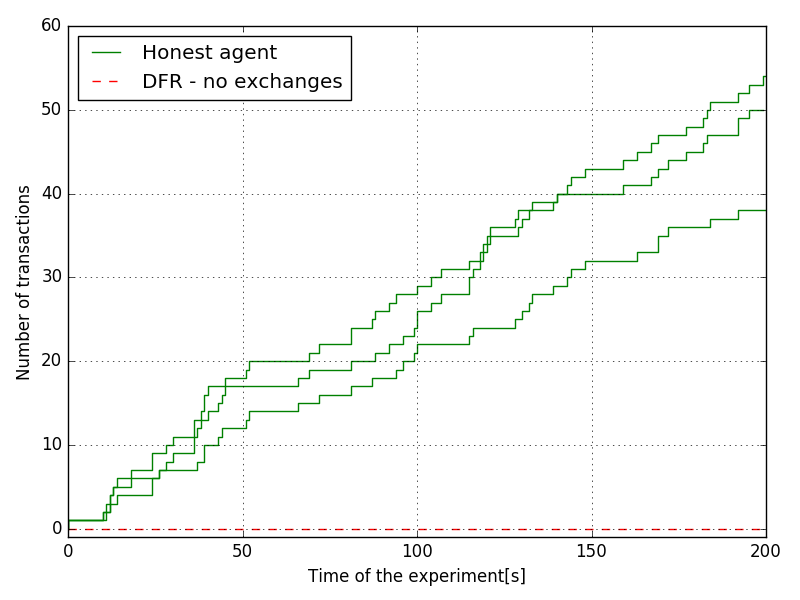
\includegraphics[width=.6\linewidth]{images/DFR_no_exchanges}
      \caption{Transactions over time of honest agents with dissemination free-rider that does not 
      perform any exchanges}
      \label{fig:DFR_no_exchanges}
    \end{subfigure}\\
    \begin{subfigure}{\textwidth}
      \centering
      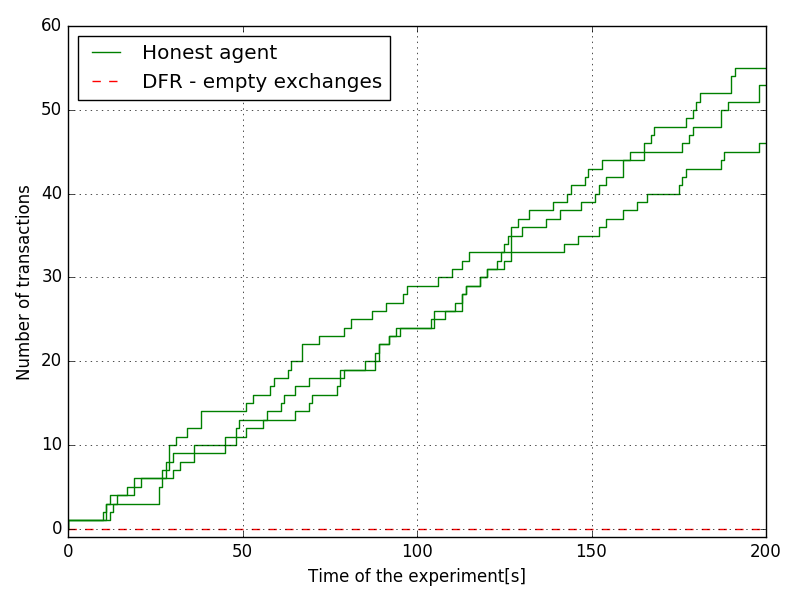
\includegraphics[width=.6\linewidth]{images/DFR_empty_exchanges}
      \caption{Transactions over time of honest agents with dissemination free-rider that creates 
      empty exchanges}
      \label{fig:DFR_empty_exchanges}
    \end{subfigure}\\
    \begin{subfigure}{\textwidth}
        \centering
        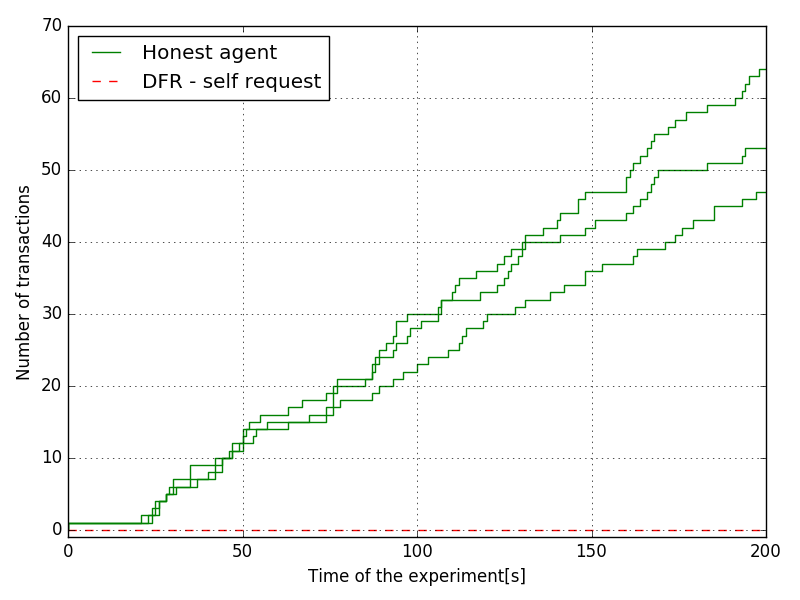
\includegraphics[width=.6\linewidth]{images/DFR_self_request}
        \caption{Transactions over time of honest agents with dissemination free-rider that only 
        exchanges own data}
        \label{fig:DFR_self_request}
      \end{subfigure}
\end{figure}

\subsection{Collaborating dissemination free-riders}

\begin{figure}[h!]
    \centering
    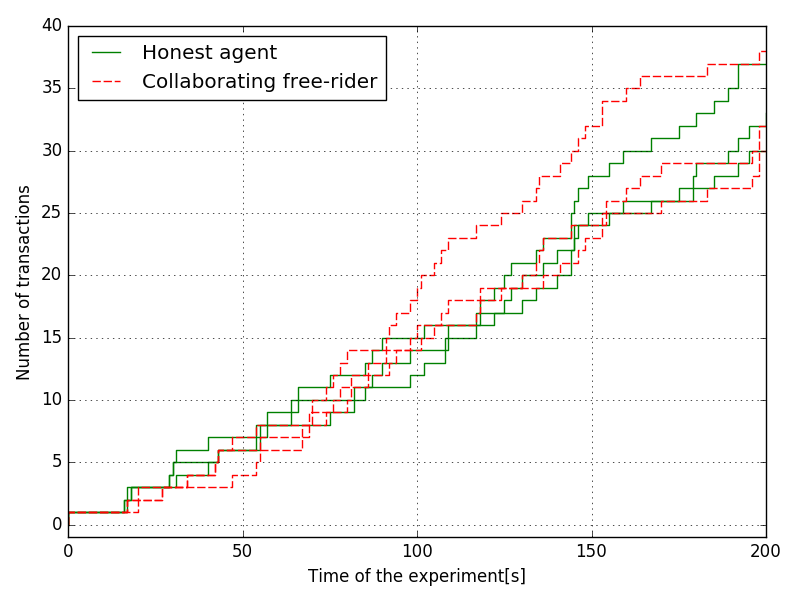
\includegraphics[width=0.7\textwidth]{images/50percent}
    \caption{Transaction history of three honest agents and three dissemination free-riders
    that are cooperating}
    \label{fig:50percent}
\end{figure}

\begin{figure}[h!]
    \centering
    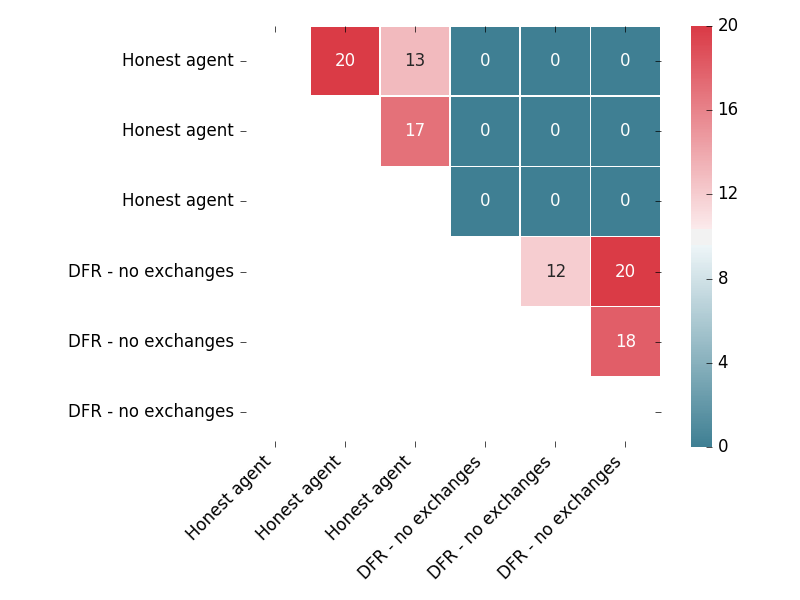
\includegraphics[width=0.7\textwidth]{images/50percent_interaction_matrix}
    \caption{Interaction matrix of three honest agents and three dissemination free-riders who are cooperating}
    \label{fig:50percent}
\end{figure}

\subsection{Malicious behavior}

\begin{figure}
    \begin{subfigure}{\textwidth}
      \centering
      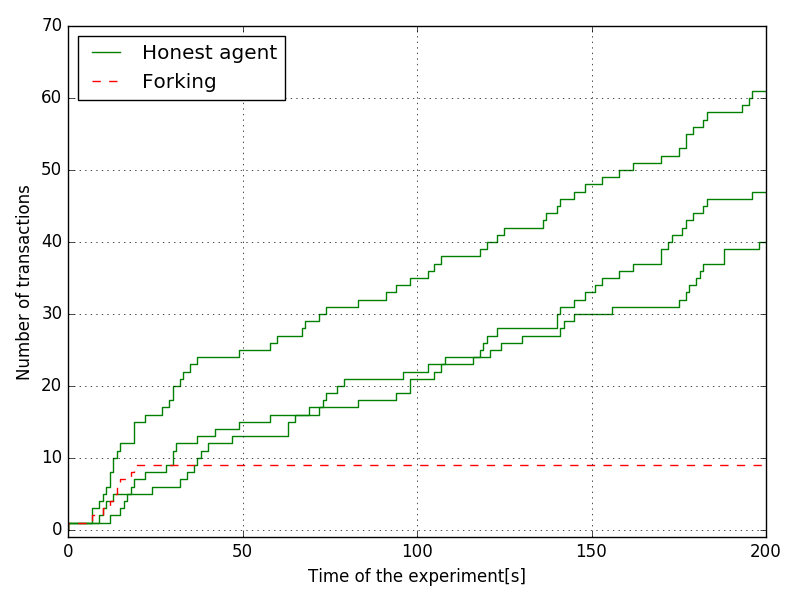
\includegraphics[width=.6\linewidth]{images/forking}
      \caption{Transaction history of three honest agents interacting with one strategic manipulator who performs a fork}
      \label{fig:forking}
    \end{subfigure}\\
    \begin{subfigure}{\textwidth}
      \centering
      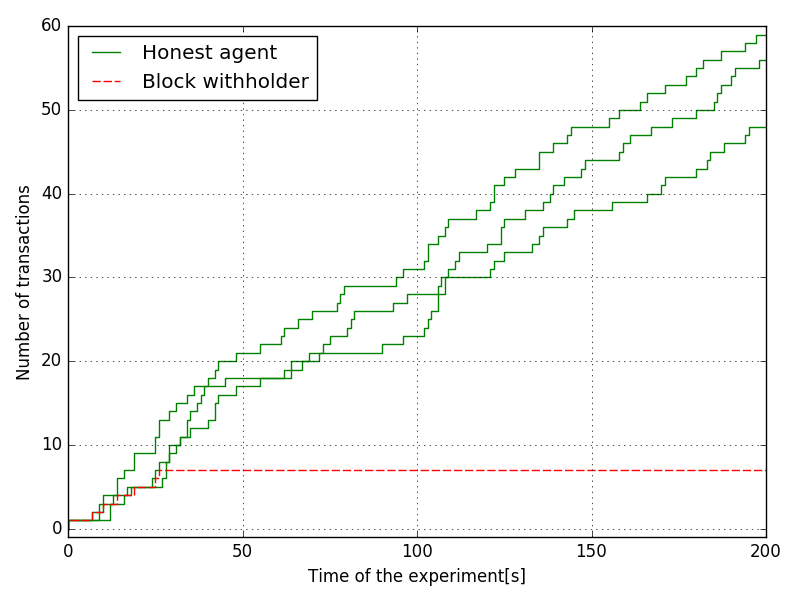
\includegraphics[width=.6\linewidth]{images/transaction_hiding}
      \caption{Transactions over time of three honest agents with one strategic manipulator who tries to hide a transaction}
      \label{fig:DFR_empty_exchanges}
    \end{subfigure}\\
\end{figure}

\subsection{Verification free-rider}

\begin{figure}
    \begin{subfigure}{\textwidth}
      \centering
      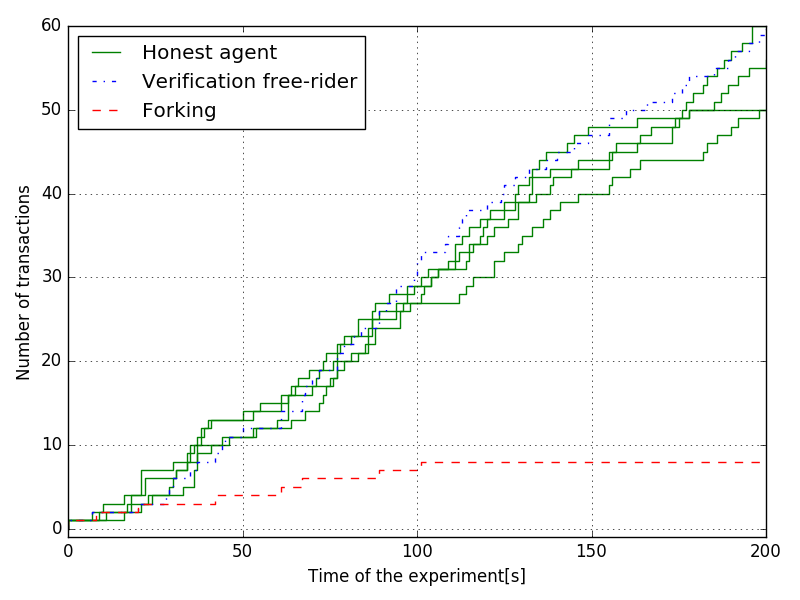
\includegraphics[width=.6\linewidth]{images/verification_doublespend_honest}
      \caption{Transaction history of three honest agents interacting with one strategic manipulator who performs a fork and a verification free-rider}
      \label{fig:verification_doublespend_honest}
    \end{subfigure}\\
    \begin{subfigure}{\textwidth}
      \centering
      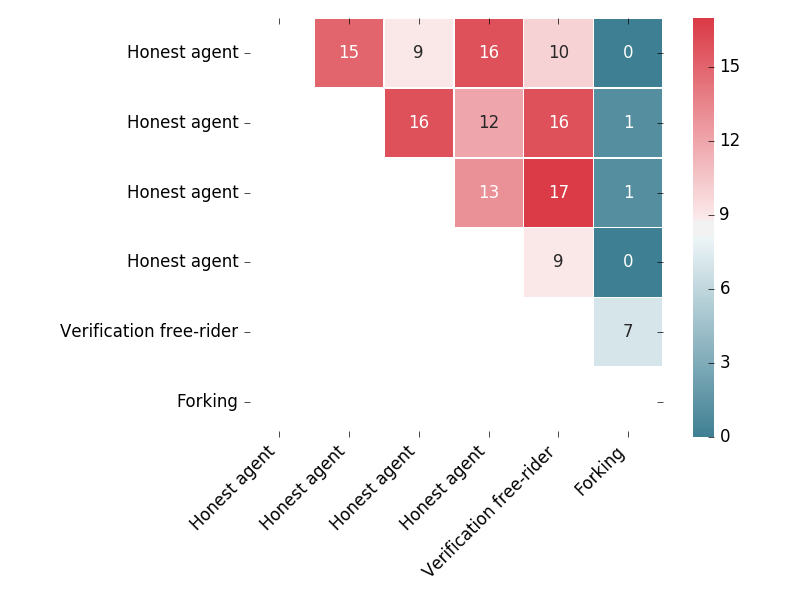
\includegraphics[width=.6\linewidth]{images/verification_doublespend_honest_matrix}
      \caption{Interaction matrix of three honest agents with one strategic manipulator who performs a fork and a verification free-rider}
      \label{fig:verification_doublespend_honest_matrix}
    \end{subfigure}\\
\end{figure}

\begin{figure}
    \begin{subfigure}{\textwidth}
      \centering
      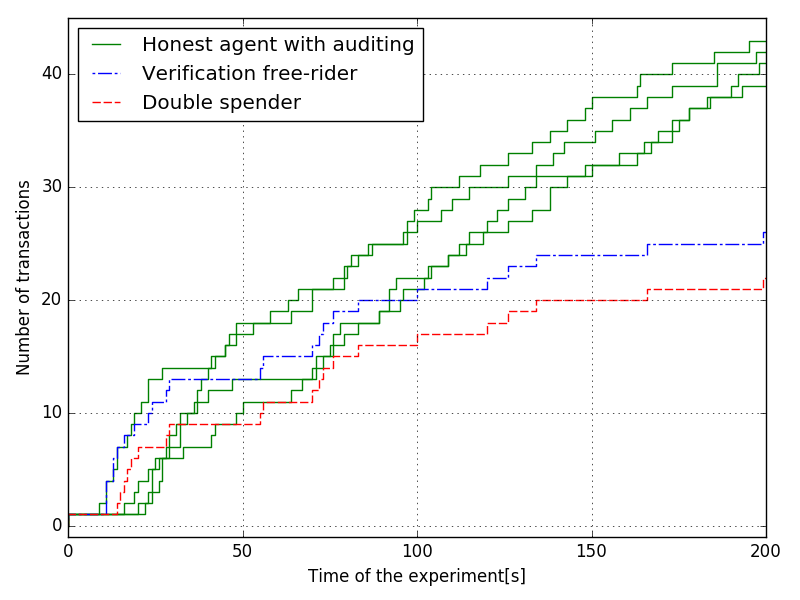
\includegraphics[width=.6\linewidth]{images/verification_doublespending}
      \caption{Transaction history of three honest agents with replay verification interacting with one strategic manipulator who performs a fork and a verification free-rider}
      \label{fig:verification_doublespending}
    \end{subfigure}\\
    \begin{subfigure}{\textwidth}
      \centering
      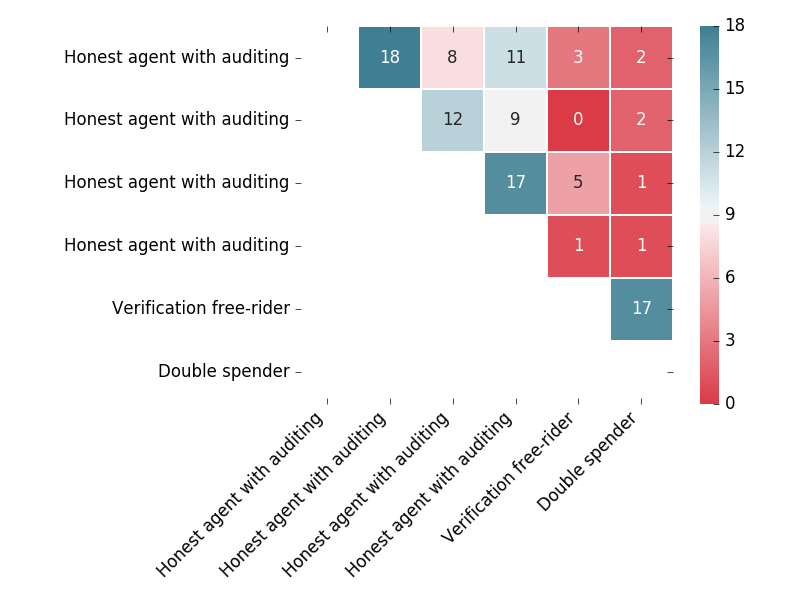
\includegraphics[width=.6\linewidth]{images/verification_doublespending_matrix}
      \caption{Interaction matrix of three honest agents with replay verification with one strategic manipulator who performs a fork and a verification free-rider}
      \label{fig:verification_doublespending_matrix}
    \end{subfigure}\\
\end{figure}

\section{}

\subsection{Sybil attack}

\chapter{Discussion}
In this work we presented a strategy-proof mechanism for information dissemination. Applied to our 
distributed blockchain based trust system we are able to effectively defend against dissemination 
and verification free-riders. It creates an incentive for each agent on the network to help defend 
the network against any lazy or malicious behavior. It thereby is a major step towards a secure, 
distributed and scalable trust system.

* we defined a new blockchain system based on TrustChain which provides internal agent state 
transparency/gossip transparency
* we formally proof that the architecture provides a complete view of the internal state of the 
agent
* we defined a specific mechanism that makes use of the archiecture
* we experimentally proof that honest agents are able to eventually identify free-riders and malicious
agents

\section{Future research}

\subsection{Further developing this mechanism}
* incremental 
* research scalability properties for this mechanism
* locality by interacting with those that have similar information
* sybil attack resistance by checking that new agents paid their dues

\subsection{Next steps for the trust system}
* locality with ping
* 

%% Use letters for the chapter numbers of the appendices.
\appendix

%\input{appendix-a}

\bibliography{report}

\end{document}

